\chapter{Dimensionnement \& Choix du matériel}
\section{Système de fixation}
Le porte-mouvement retenu est le modèle métallique industriel \No 4040 de la marque Bergeon. 
Sa large compatibilité lui permet d'accueillir l'ensemble des calibres définis dans le cahier des charges. 
Par ailleurs, son utilisation avérée dans les ateliers de Breitling atteste de son adéquation aux exigences d'un environnement de production horloger professionnel.
\begin{figure}[H]
    \centering
    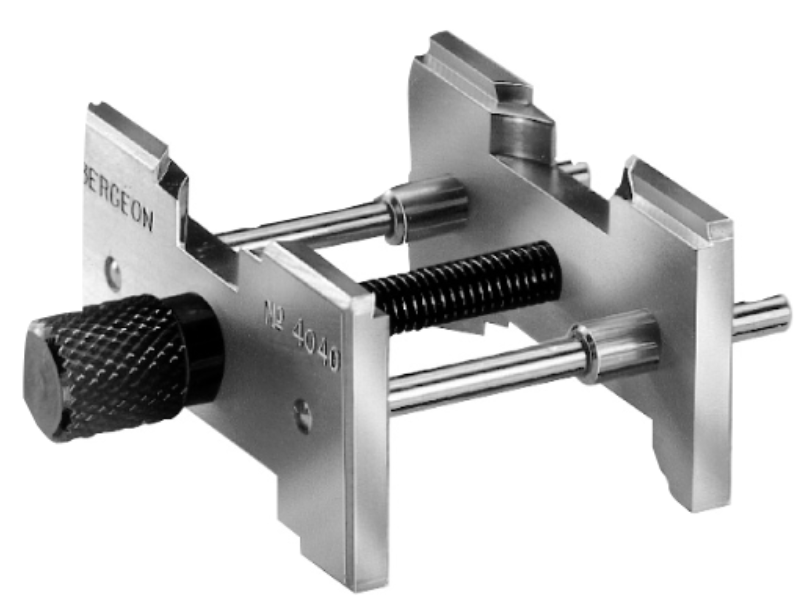
\includegraphics[width=0.5\textwidth]{assets/figures/Dimensionement/bergeon no 4040.png}
    \caption{Illustration du porte mouvement \No 4040 issue de la datasheet disponible en annexe \cite{bergeon_catalogue}}
    \label{fig:no 4040}
\end{figure}
\section{Système de motorisation}
\subsection{Choix du moteur}
\subsubsection{Modes de fonctionnement}
Le moteur constitue l'actionneur central du banc de test. 
Il doit répondre aux exigences de deux modes de fonctionnement distincts :
\begin{itemize}
    \item Mode vieillissement accéléré~: le moteur effectue des impulsions de rotation répétées, chacune inférieure à 2 tours, afin de simuler le remontage manuel d'une montre. Ces impulsions sont réalisées à une vitesse de 350 tours/min avec une accélération pouvant atteindre 5000 tours/min², ce qui impose au moteur des démarrages et arrêts dynamiques fréquents.

    \item Mode réserve de marche~: ce mode se déroule en deux phases. Dans un premier temps, le moteur entraîne la tige du mouvement à 50 tours/min pour remonter le barillet complètement puis le dévider du nombre de tours souhaité. Dans un second temps, le moteur se maintient en position bloquée pendant environ 24 heures, empêchant toute rotation du système pendant que la caméra enregistre le déroulement du barillet.
\end{itemize}
\subsubsection{Justification du choix : moteur pas à pas}
Un moteur pas à pas a été retenu. Ce choix se justifie par trois critères majeurs :
\begin{itemize}
    \setlength{\itemsep}{6pt}
    \item Contrôle précis de la position angulaire~: Le nombre de tours doit être connu avec précision. En considérant une résolution minimale requise de 0,02 tour (soit 7,2°), un moteur pas à pas standard à 200 pas/tour offre un pas de 1,8°, soit une résolution quatre fois meilleure que celle exigée.
    
    \item Maintien statique : En mode réserve de marche, la phase de blocage sur 24 heures nécessite de retenir le mouvements afin d'éviter qu'il se dévide tout seul. Les moteurs pas à pas ont un couple de détente pouvant retenir naturellement la position même une fois hors tension, ce qu'aucun autre type de moteur ne peut faire.
    
    \item Commande simple et reproductible~: Le nombre de pas envoyés détermine directement l'angle parcouru, sans calibration préalable.
\end{itemize}
\subsubsection{Sélection du format et du modèle}
Parmi les formats normalisés de moteurs pas à pas à 200 pas/tour, il existe plusieurs tailles différentes (NEMA 8, NEMA 11, NEMA 17). 
Le format NEMA 11 a été retenu pour optimiser la compacité.
\begin{figure}[H]
    \centering
    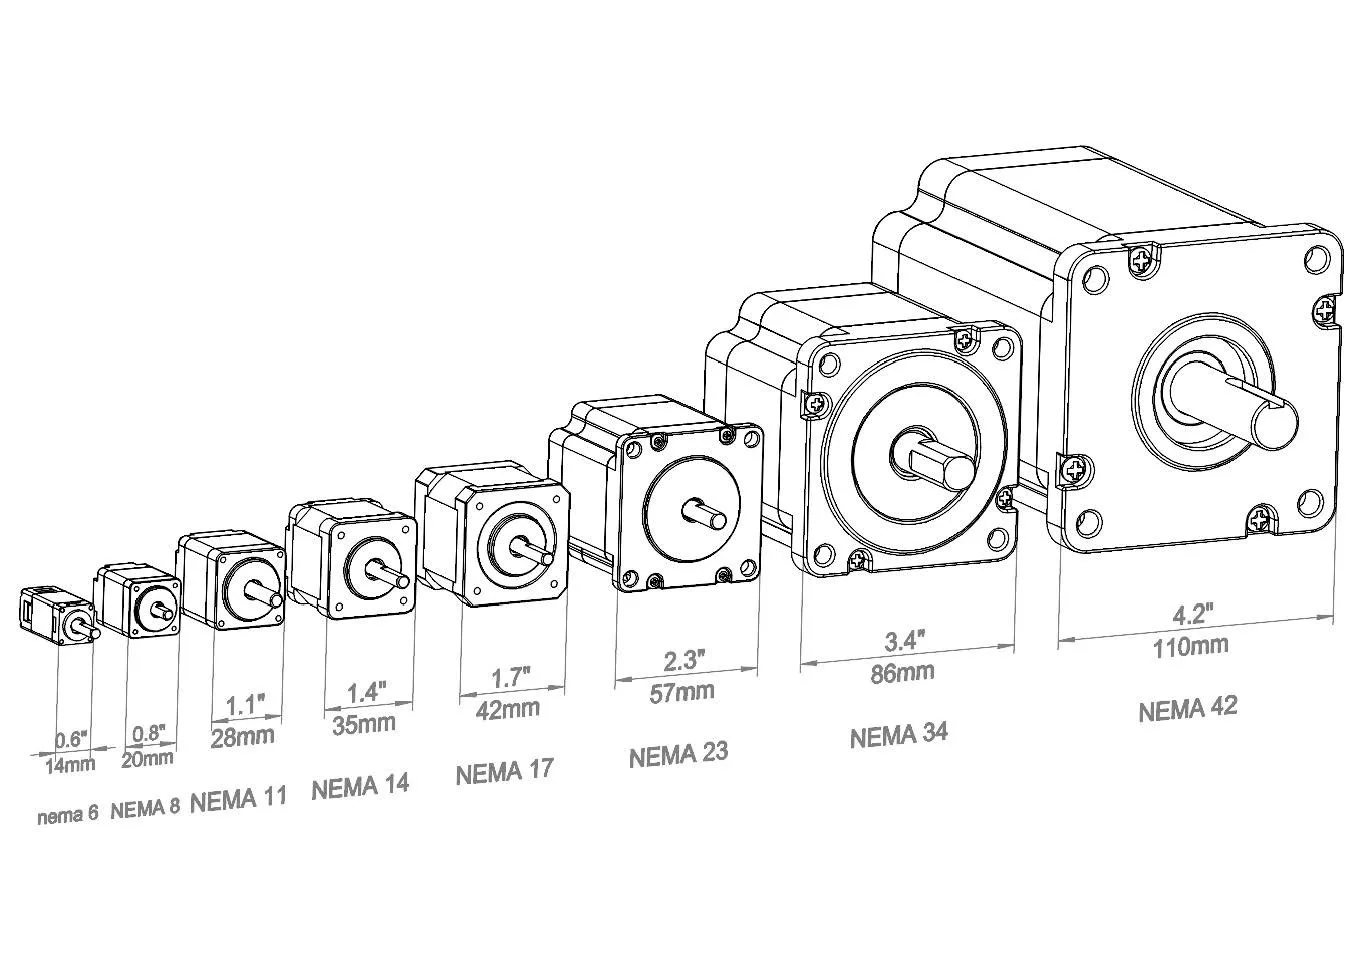
\includegraphics[width=1\textwidth]{assets/figures/Dimensionement/tailleNEMA.png}
    \caption{Illustration des différentes tailles de moteur pas à pas \cite{NEMA_taille}}
    \label{fig:taille_NEMA}
\end{figure}
D'après les données techniques fournies, le couple maximal que le barillet peut exercer est de 10,8 mN·m. 
Compte tenu d'un rapport de réduction de 3,33 entre la tige et le barillet, le couple que le moteur doit exercer pour remonter le mouvement est de 3,24 mN·m. 
En appliquant une marge de sécurité pour les frottements mécaniques et les variations de charge, le couple maximal à appliquer sur la tige du mouvement pour le remonter est fixé à :
\begin{equation}
    C_{\text{tige}} = 4 \text{ mN·m}
    \label{eq:couple_tige}
\end{equation}
$C_{\text{tige}}$ est également le couple minimal requis au niveau de la tige pour maintenir le système et éviter qu'il se décharge spontanément sous l'effet du ressort.
Pour le calcul du couple dynamique, le moment d'inertie de la fourche en T est estimé à 8,67~g·cm²  et celui de la fourche en U à XXX~g·cm² d'après le logiciel SolidWorks. 
L'inertie complète de l'accouplement vaut donc :
\begin{equation}
    J_{\text{accouplement}} = 15 \text{g·cm²}
    \label{eq:inertie_accouplement}
\end{equation}
L'accélération angulaire maximale de 5000~tr/min² est convertie en unités SI :
\begin{equation}
    \alpha = 5000 \frac{\text{tr}}{\text{min}^2} \times \frac{2\pi}{\text{tr}} 
    \times \frac{1}{3600} \frac{\text{min}^2}{\text{s}^2} \approx 8{,}73 \text{ rad/s}^2
    \label{eq:alpha}
\end{equation}
\noindent Le couple dynamique requis est donc :
\begin{equation}
    C_{\text{dynamique}} = J_{\text{accouplement}} \times \alpha 
    = 15 \times 10^{-7} \times 8{,}73 
    \approx 1{,}31 \times 10^{-5} \text{ N·m} 
    = 0{,}013 \text{ mN·m}
    \label{eq:couple_dynamique}
\end{equation}
\noindent où $J_{\text{accouplement}} = 15~\text{g·cm}^2 = 15 \times 10^{-7}~\text{kg·m}^2$ et $\alpha \approx 8{,}73~\text{rad/s}^2$. Cette valeur est négligeable au vu de son ordre de grandeur. 
On cherche donc un moteur pas à pas de format NEMA 11 ayant un couple de détente supérieur au couple tige.
Finalement, le moteur retenu est le NEMA11-01 de Joy-IT (référence 28SHD4201-20) \cite{moons_nema11, joytechnik_nema11_01}. Ses caractéristiques principales sont présentées au tableau~\ref{tab:specs_moteur}:
\begin{figure}[H]
    \centering
    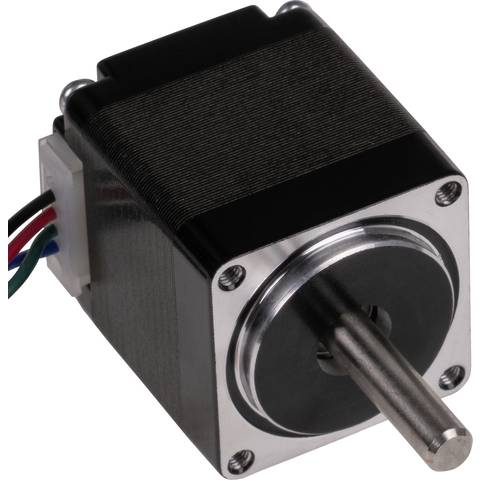
\includegraphics[width=0.4\textwidth]{assets/figures/Dimensionement/Moteur Nema11-01.jpg}
    \caption{Moteur pas à pas NEMA11-01 de Joy-IT \cite{joytechnik_nema11_01}}
    \label{fig:moteur_nema11}
\end{figure}
\begin{table}[H]
  \centering
  \caption{Caractéristiques du moteur pas à pas NEMA11-01}
  \label{tab:specs_moteur}
  \begin{tabular}{ll}
    \toprule
    \textbf{Paramètre} & \textbf{Valeur} \\
    \midrule
    Couple de maintien & 55 mN·m \\
    Couple de détente & 5 mN·m \\
    Courant nominal & 0,42 A \\
    Tension nominale & 5,0 V \\
    Angle de pas & 1,8° $\pm$ 5\% \\
    Résistance de phase & 11,9 Ω \\
    Inductance de phase & 7,8 mH \\
    \bottomrule
  \end{tabular}
\end{table}
La courbe couple-vitesse a été établie en se référant aux données du fabricant MOONS', dont les moteurs présentent des spécifications électriques et mécaniques similaires au NEMA11-01. L'étudiant a fait ce choix, car le fabricant ne fournissait pas la courbe couple-vitesse de son moteur.
\begin{figure}[H]
    \centering
    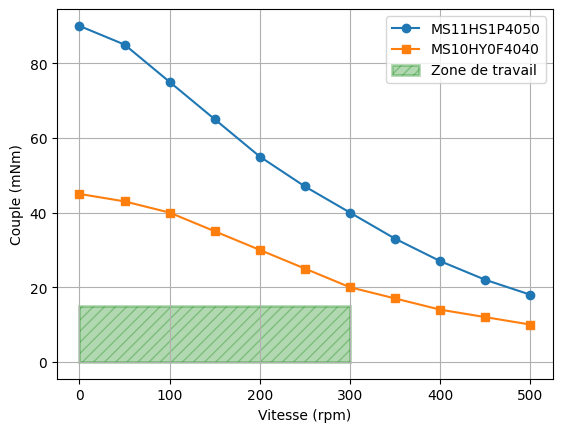
\includegraphics[width=1\textwidth]{assets/figures/Dimensionement/graphe courbe couple vitesse moteur.png}
    \caption{Courbes couple-vitesse des moteurs NEMA}
    \label{fig:couple_vitesse}
\end{figure}
\subsection{Choix du driver}
\subsubsection{Critères de sélection}
Le driver doit satisfaire trois critères~: la compatibilité mécanique avec le moteur, une plage de courant adaptée à la précision requise, et la capacité à piloter plusieurs axes depuis un ordinateur.
\subsubsection{Compatibilité mécanique}
Le moteur NEMA 11 a des dimensions de 28 x 28 mm. 
Le driver doit être montable directement à l'arrière d'un tel moteur.
\subsubsection{Calculs des couples}

Plusieurs couples distincts interviennent dans le dimensionnement du système de motorisation. Il est important de bien les distinguer afin de garantir la sécurité du mouvement.

Pour commencer, il y a le couple de détente $C_{\text{détente}}$. Il s'agit d'un couple résistif généré par les aimants permanents du moteur, présent qu'il soit alimenté ou non. 
Il s'oppose à toute rotation et représente le seuil minimal à franchir pour que l'arbre du moteur commence à tourner, ce dernier est donné par le fabricant dans la datasheet du moteur :
\begin{equation}
    C_{\text{détente}} = 5 \text{ mN·m}
    \label{eq:couple_detente}
\end{equation}

Ensuite, il y a le couple tige $C_{\text{tige}}$. C'est un couple additionnel que le moteur doit transmettre à la tige pour entraîner le mouvement, c'est-à-dire vaincre le couple du barillet ramené sur la tige. La valeur est calculée pour chaque mouvement :
\begin{equation}
    C_{\text{tige}} = \frac{C_{\text{barillet}}}{r}
    \label{eq:couple_tige_formule}
\end{equation}
Le tableau~\ref{tab:couple_tige} présente les résultats pour l'ensemble des mouvements.

\begin{table}[H]
  \centering
  \caption{Couple tige calculé pour chaque mouvement}
  \label{tab:couple_tige}
  \begin{tabular}{|c|c|c|c|}
    \hline
    \textbf{Mouvement} & $\boldsymbol{C_{\text{barillet}}}$ \textbf{[mN·m]} & $\boldsymbol{r}$ \textbf{(tige/bar.)} & $\boldsymbol{C_{\text{tige}}}$ \textbf{[mN·m]} \\
    \hline
    Mvt19    & 6,7  & 3,33 & 2,01 \\
    Mvt01    & 10,8 & 3,33 & 3,24 \\
    Mvt200   & 7,9  & 3,33 & 2,37 \\
    Mvt200.1 & 7,9  & 3,33 & 2,37 \\
    Mvt110   & 6,81 & 2,84 & 2,40 \\
    Mvt111   & 4,06 & 2,96 & 1,37 \\
    \hline
  \end{tabular}
\end{table}

Le cas critique est le Mvt01 ($C_{\text{barillet}} = 10{,}8$ mN·m, $r = 3{,}33$), qui donne le $C_{\text{tige}}$ le plus élevé :
\begin{equation}
    C_{\text{tige}} = \frac{C_{\text{barillet,max}}}{r}
    = \frac{10{,}8}{3{,}33}
    \approx 3{,}24 \text{ mN·m}
    \label{eq:couple_tige_calc}
\end{equation}

De plus, il y a le couple maximal admissible sur la tige $C_{\text{max,tige}}$. C'est-à-dire, le Couple maximal autorisé sur la tige de remontoir, imposé par le cahier des charges( FC1, E1) afin d'éviter tout dommage mécanique au mouvement :
\begin{equation}
    C_{\text{max,tige}} = 15 \text{ mN·m}
    \label{eq:couple_max_tige}
\end{equation}

Mais aussi, le Couple de maintien du moteur $C_{\text{maintien}}$. Le Couple maximal développé par le moteur à vitesse nulle, dans les conditions nominales données par le fabricant dans la datasheet :
\begin{equation}
    C_{\text{maintien}} = 55 \text{ mN·m}
    \label{eq:couple_maintien_moteur}
\end{equation}

Enfin, il y a le couple fourni par le moteur $C_{\text{moteur}}$, c'est-à-dire
le couple effectivement délivré par le moteur, dont la valeur dépend du
réglage du driver.

À partir de ces valeurs, on définit le couple requis $C_{\text{requis}}$,
c'est-à-dire le couple que le moteur doit délivrer pour entraîner
effectivement le mouvement :
\begin{equation}
    C_{\text{requis}} = C_{\text{tige}} + C_{\text{détente}}
    \label{eq:couple_requis_def}
\end{equation}
\noindent $C_{\text{requis}}$ dépendant de $C_{\text{tige}}$, sa valeur est propre à chaque mouvement. Le tableau~\ref{tab:couple_requis} présente les résultats pour l'ensemble des mouvements.

\begin{table}[H]
  \centering
  \caption{Couple requis calculé pour chaque mouvement}
  \label{tab:couple_requis}
  \begin{tabular}{|c|c|c|c|}
    \hline
    \textbf{Mouvement} & $\boldsymbol{C_{\text{tige}}}$ \textbf{[mN·m]} & $\boldsymbol{C_{\text{détente}}}$ \textbf{[mN·m]} & $\boldsymbol{C_{\text{requis}}}$ \textbf{[mN·m]} \\
    \hline
    Mvt19    & 2,01 & 5 & 7,01 \\
    Mvt01    & 3,24 & 5 & 8,24 \\
    Mvt200   & 2,37 & 5 & 7,37 \\
    Mvt200.1 & 2,37 & 5 & 7,37 \\
    Mvt110   & 2,40 & 5 & 7,40 \\
    Mvt111   & 1,37 & 5 & 6,37 \\
    \hline
  \end{tabular}
\end{table}

La plage de couple utile est alors définie de la manière suivante~: tant que
$C_{\text{moteur}} < C_{\text{requis}}$, le couple transmis à la tige est
insuffisant pour affirmer avec certitude que l'on peut entraîner le
mouvement. Au-delà, $C_{\text{moteur}}$ entraîne activement la tige,
permettant le remontage ou le dévidage contrôlé du barillet, jusqu'à la
limite de sécurité $C_{\text{max,tige}}$.

Plus précisément, entre $C_{\text{détente}}$ et $C_{\text{requis}}$ se
trouve une zone incertaine. En effet, $C_{\text{requis}}$ est
calculé pour le cas critique, c'est-à-dire pour le couple \emph{maximal} du
barillet (ressort complètement armé). Le couple réellement opposé par le
barillet dépend cependant de son état d'armage et peut être nettement plus
faible à d'autres moments de la réserve de marche. Il n'est donc pas garanti
qu'un couple moteur inférieur à $C_{\text{requis}}$ n'entraîne pas le
mouvement~: selon l'état du ressort, l'entraînement peut débuter à un couple
plus faible, ce qui rend cette zone incertaine plutôt que strictement dédiée
à un accouplement sans entraînement.

La figure~\ref{fig:plages_couples} illustre, pour chaque mouvement, la
position de ces valeurs et les zones de fonctionnement correspondantes, à
l'échelle.

\newcommand{\graphePlageCouple}[3]{%
\begin{tikzpicture}[font=\tiny]
  \def\k{0.68}
  \pgfmathsetmacro{\xdet}{5*\k}
  \pgfmathsetmacro{\xreq}{#1*\k}
  \pgfmathsetmacro{\xmax}{15*\k}
  \pgfmathsetmacro{\xend}{20*\k}
  \pgfmathsetmacro{\xaxisend}{\xend+0.6}

  \fill[gray!30]   (0,0.35) rectangle (\xdet,0.95);
  \fill[orange!25] (\xdet,0.35) rectangle (\xreq,0.95);
  \fill[green!25]  (\xreq,0.35) rectangle (\xmax,0.95);
  \fill[red!15]    (\xmax,0.35) rectangle (\xend,0.95);
  \draw (0,0.35) rectangle (\xdet,0.95);
  \draw (\xdet,0.35) rectangle (\xreq,0.95);
  \draw (\xreq,0.35) rectangle (\xmax,0.95);
  \draw (\xmax,0.35) rectangle (\xend,0.95);

  \ifnum#3=1
  \foreach \ccs in {2.86, 5.83, 8.69, 11.55, 14.52, 17.38} {
    \pgfmathsetmacro{\xcs}{\ccs*\k}
    \draw[dashed] (\xcs,0.35) -- (\xcs,0.95);
  }
  \fi

  \draw[->, thick] (0,0) -- (\xaxisend,0) node[right] {[mN·m]};

  \draw (0,0.15) -- (0,-0.15);
  \node[below] at (0,-0.2) {0};
  \draw (\xdet,0.15) -- (\xdet,-0.15);
  \node[below] at (\xdet,-0.2) {5};
  \draw (\xreq,0.15) -- (\xreq,-0.15);
  \node[below] at (\xreq,-0.2) {#2};
  \draw (\xmax,0.15) -- (\xmax,-0.15);
  \node[below] at (\xmax,-0.2) {15};
\end{tikzpicture}%
}

\begin{figure}[H]
  \centering
  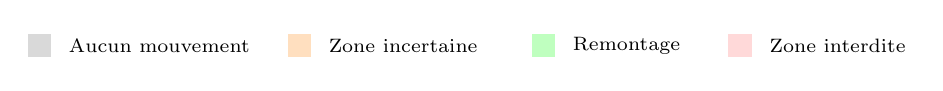
\begin{tikzpicture}[font=\scriptsize, baseline]
    \fill[gray!30]   (0,0)   rectangle (0.3,0.3); \node[anchor=west] at (0.4,0.15) {Aucun mouvement};
    \fill[orange!25] (3.3,0) rectangle (3.6,0.3); \node[anchor=west] at (3.7,0.15) {Zone incertaine};
    \fill[green!25]  (6.4,0) rectangle (6.7,0.3); \node[anchor=west] at (6.8,0.15) {Remontage};
    \fill[red!15]    (8.9,0) rectangle (9.2,0.3); \node[anchor=west] at (9.3,0.15) {Zone interdite};
  \end{tikzpicture}\\[3mm]
  \textbf{Mvt19}\\[1mm]
  \graphePlageCouple{7.01}{7,01}{0}\\[3mm]
  \textbf{Mvt01}\\[1mm]
  \graphePlageCouple{8.24}{8,24}{0}\\[3mm]
  \textbf{Mvt200}\\[1mm]
  \graphePlageCouple{7.37}{7,37}{0}\\[3mm]
  \textbf{Mvt200.1}\\[1mm]
  \graphePlageCouple{7.37}{7,37}{0}\\[3mm]
  \textbf{Mvt110}\\[1mm]
  \graphePlageCouple{7.40}{7,40}{0}\\[3mm]
  \textbf{Mvt111}\\[1mm]
  \graphePlageCouple{6.37}{6,37}{0}
  \caption{Plage de couple opérationnelle du moteur pour chaque mouvement}
  \label{fig:plages_couples}
\end{figure}

Cette plage de fonctionnement n'est exploitable que si la résolution du driver est suffisante pour positionner le couple avec précision.

\subsubsection{Régulation de courant}

Le driver TMCM-1021 ne régule pas le courant par asservissement logiciel~:
un \emph{chopper} intégré au driver module le courant en largeur
d'impulsion (PWM) directement sur la puce, en boucle fermée interne. Le
logiciel se limite à écrire une consigne dans le registre CS
(\emph{Current Scale}) via le protocole TMCL. Ce registre offre 32 niveaux
discrets ($CS \in \{0, \ldots, 31\}$, soit 5~bits de résolution)~: il ne
s'agit donc pas d'un réglage continu, mais d'une contrainte matérielle du
driver.

Le courant efficace correspondant à chaque palier est donné par le
fabricant \cite{trinamic_tmcm_1021}~:
\begin{equation}
    I_{\text{RMS}}(CS) = \frac{CS+1}{32} \times \frac{I_{\text{pleine\,échelle}}}{\sqrt{2}}
    \label{eq:irms_cs}
\end{equation}
\noindent où $I_{\text{pleine\,échelle}} = 1{,}1$ A est le courant de crête
maximal du driver en plage basse.

Le couple de maintien $C_{\text{maintien}} = 55$~mN·m est atteint au palier
nominal $CS = 18$, ce qui correspond, d'après l'équation~\eqref{eq:irms_cs},
à un courant de référence~:
\begin{equation}
    I_{\text{RMS}}(18) = \frac{19}{32} \times \frac{1{,}1}{\sqrt{2}} \approx 0{,}462 \text{ A}
    \label{eq:irms_18}
\end{equation}

En supposant le couple proportionnel au courant, le couple délivré par le
moteur pour un palier $CS$ quelconque s'approxime alors par~:
\begin{equation}
    C_{\text{moteur}}(CS) = \frac{I_{\text{RMS}}(CS)}{I_{\text{RMS}}(18)} \times C_{\text{maintien}}
    = \frac{CS+1}{19} \times C_{\text{maintien}}
    \label{eq:couple_moteur_cs}
\end{equation}

À titre de vérification, le palier $CS = 0$ donne~:
\begin{equation}
    C_{\text{moteur}}(0) = \frac{1}{19} \times 55 \approx 2{,}9 \text{ mN·m}
    \label{eq:couple_moteur_cs0}
\end{equation}
\noindent ce qui constitue un plancher physique incompressible~: même au
palier le plus bas, le moteur délivre déjà un couple non nul, en dessous
duquel il n'est pas possible de descendre en pilotant uniquement le
registre CS.

Le tableau~\ref{tab:echelons_couple} applique l'équation~\eqref{eq:couple_moteur_cs}
à l'ensemble des 32 paliers, avec les valeurs de courant réelles publiées
par le fabricant \cite{trinamic_tmcm_1021}.

\begin{longtable}{|c|c|c|c|}
  \caption{Courant et couple moteur pour chaque palier du driver \cite{trinamic_tmcm_1021}}
  \label{tab:echelons_couple}\\
  \hline
  \textbf{Palier (CS)} & \textbf{Valeur TMCL} & \textbf{Courant $I_{\text{RMS}}$ [A]} & \textbf{$C_{\text{moteur}}$ [mN·m]} \\
  \hline
  \endfirsthead
  \hline
  \textbf{Palier (CS)} & \textbf{Valeur TMCL} & \textbf{Courant $I_{\text{RMS}}$ [A]} & \textbf{$C_{\text{moteur}}$ [mN·m]} \\
  \hline
  \endhead
  0  & 0--7     & 0,024 & 2,86  \\
  1  & 8--15    & 0,049 & 5,83  \\
  2  & 16--23   & 0,073 & 8,69  \\
  3  & 24--31   & 0,097 & 11,55 \\
  4  & 32--39   & 0,122 & 14,52 \\
  5  & 40--47   & 0,146 & 17,38 \\
  6  & 48--55   & 0,170 & 20,24 \\
  7  & 56--63   & 0,194 & 23,10 \\
  8  & 64--71   & 0,219 & 26,07 \\
  9  & 72--79   & 0,243 & 28,93 \\
  10 & 80--87   & 0,267 & 31,79 \\
  11 & 88--95   & 0,292 & 34,76 \\
  12 & 96--103  & 0,316 & 37,62 \\
  13 & 104--111 & 0,340 & 40,48 \\
  14 & 112--119 & 0,365 & 43,45 \\
  15 & 120--127 & 0,389 & 46,31 \\
  16 & 128--135 & 0,413 & 49,17 \\
  17 & 136--143 & 0,438 & 52,14 \\
  18 & 144--151 & 0,462 & 55,00 \\
  19 & 152--159 & 0,486 & 57,86 \\
  20 & 160--167 & 0,510 & 60,71 \\
  21 & 168--175 & 0,535 & 63,69 \\
  22 & 176--183 & 0,559 & 66,55 \\
  23 & 184--191 & 0,583 & 69,40 \\
  24 & 192--199 & 0,608 & 72,38 \\
  25 & 200--207 & 0,632 & 75,24 \\
  26 & 208--215 & 0,656 & 78,10 \\
  27 & 216--223 & 0,681 & 81,07 \\
  28 & 224--231 & 0,705 & 83,93 \\
  29 & 232--239 & 0,729 & 86,79 \\
  30 & 240--247 & 0,754 & 89,76 \\
  31 & 248--255 & 0,778 & 92,62 \\
  \hline
\end{longtable}

Dans la plage de fonctionnement utile (0 à 20~mN·m), seuls les paliers
$CS = 0$ à $5$ sont atteignables. La figure~\ref{fig:plages_couples_paliers}
reprend les graphiques de la figure~\ref{fig:plages_couples} en y ajoutant,
en traitillé, la position de ces paliers.

\begin{figure}[H]
  \centering
  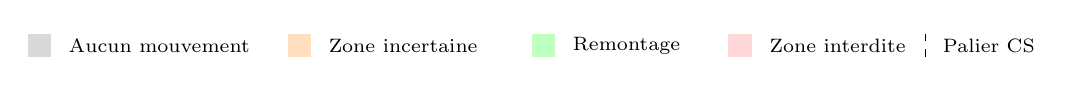
\begin{tikzpicture}[font=\scriptsize, baseline]
    \fill[gray!30]   (0,0)   rectangle (0.3,0.3); \node[anchor=west] at (0.4,0.15) {Aucun mouvement};
    \fill[orange!25] (3.3,0) rectangle (3.6,0.3); \node[anchor=west] at (3.7,0.15) {Zone incertaine};
    \fill[green!25]  (6.4,0) rectangle (6.7,0.3); \node[anchor=west] at (6.8,0.15) {Remontage};
    \fill[red!15]    (8.9,0) rectangle (9.2,0.3); \node[anchor=west] at (9.3,0.15) {Zone interdite};
    \draw[dashed] (11.4,0) -- (11.4,0.3); \node[anchor=west] at (11.5,0.15) {Palier CS};
  \end{tikzpicture}\\[3mm]
  \textbf{Mvt19}\\[1mm]
  \graphePlageCouple{7.01}{7,01}{1}\\[3mm]
  \textbf{Mvt01}\\[1mm]
  \graphePlageCouple{8.24}{8,24}{1}\\[3mm]
  \textbf{Mvt200}\\[1mm]
  \graphePlageCouple{7.37}{7,37}{1}\\[3mm]
  \textbf{Mvt200.1}\\[1mm]
  \graphePlageCouple{7.37}{7,37}{1}\\[3mm]
  \textbf{Mvt110}\\[1mm]
  \graphePlageCouple{7.40}{7,40}{1}\\[3mm]
  \textbf{Mvt111}\\[1mm]
  \graphePlageCouple{6.37}{6,37}{1}
  \caption{Plage de couple opérationnelle du moteur pour chaque mouvement, avec position des paliers CS}
  \label{fig:plages_couples_paliers}
\end{figure}

Pour le cas critique (Mvt01), seuls les paliers 2 et 3 se situent dans la
zone de remontage~; le palier 1 ($C_{\text{moteur}} \approx 5{,}8$~mN·m) se
situe quant à lui dans la zone incertaine.

\subsubsection{Driver sélectionné : TMCM-1021}
Le TMCM-1021 a été retenu \cite{trinamic_tmcm_1021}. Ses caractéristiques principales sont présentées au tableau~\ref{tab:specs_driver}:
\begin{figure}[H]
    \centering
    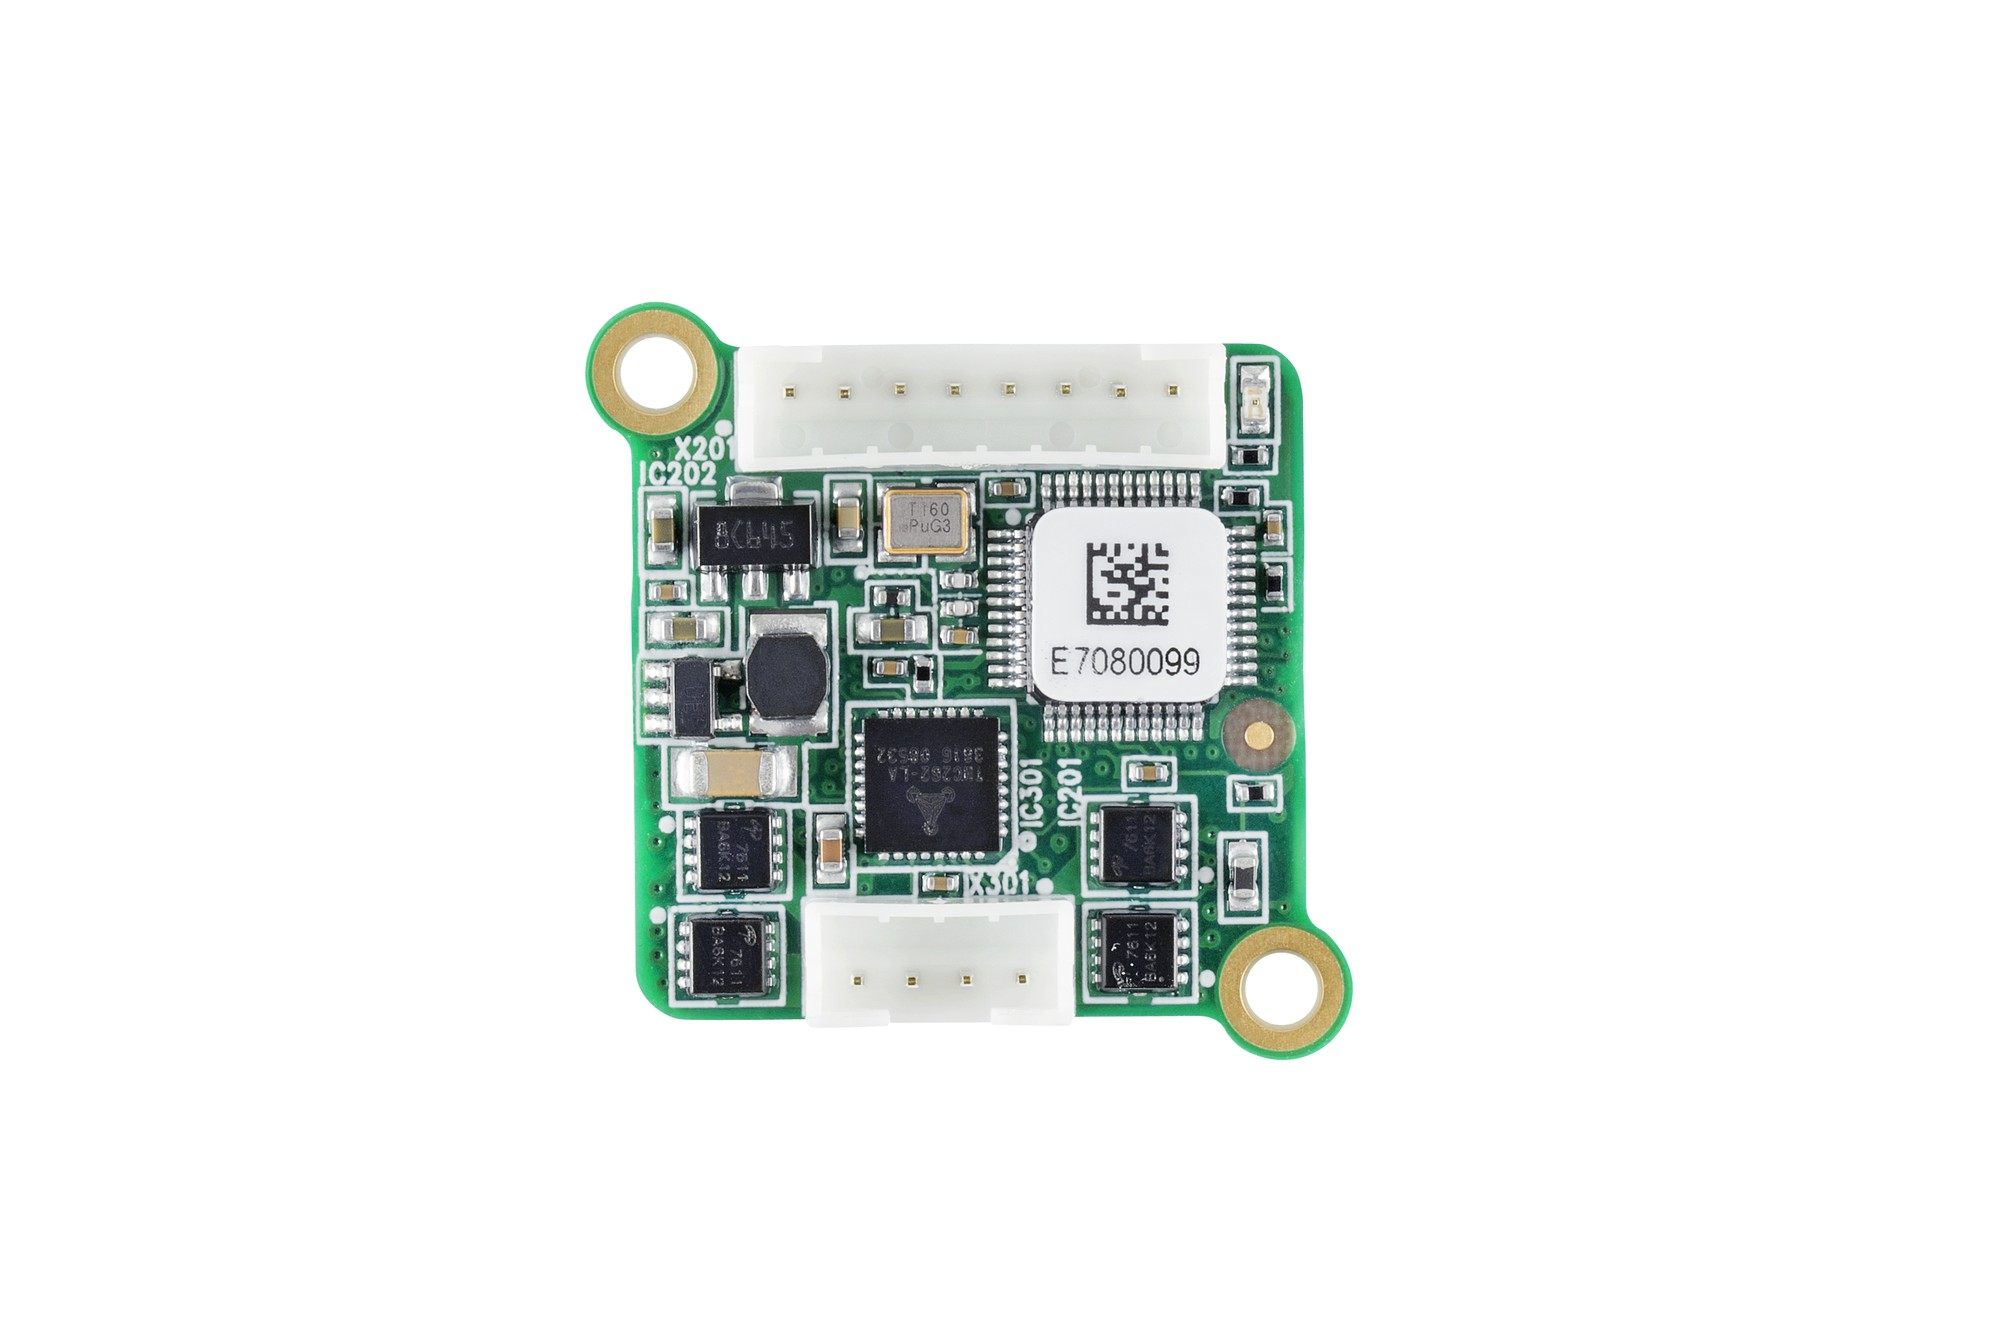
\includegraphics[width=0.8\textwidth]{assets/figures/Dimensionement/tmcm-1021.jpg}
    \caption{Driver de moteur pas à pas TMCM-1021 \cite{trinamic_tmcm_1021}}
    \label{fig:tmcm_1021}
\end{figure}
\begin{table}[H]
  \centering
  \caption{Caractéristiques du driver TMCM-1021}
  \label{tab:specs_driver}
  \begin{tabular}{ll}
    \toprule
    \textbf{Paramètre} & \textbf{Valeur} \\
    \midrule
    Format & 28 x 28 mm (NEMA 11) \\
    Plage de courant basse & 0,7 A RMS (programmable) \\
    Tension d'alimentation & 9 à 28 V \\
    Interface de communication & RS485 (protocole TMCL) \\
    Capteur intégré & SensOstep (encodeur magnétique) \\
    Fonctionnalités avancées & stallGuard2, coolStep, stealthChop \\
    \bottomrule
  \end{tabular}
\end{table}
\subsubsection{Avantages du TMCM-1021}
\begin{itemize}
    \item Pilotage multi-axes~: Le bus RS485 permet de connecter jusqu'à 255 modules sur un seul câble. Chaque driver se voit attribuer une adresse unique, permettant au script Python de les commander indépendamment via un simple adaptateur USB/RS485. Cette architecture est adaptée à une évolution vers un système multi-axes.
    
    \item Interface série~: Le TMCM-1021 peut être contrôlé directement depuis un script Python sans microcontrôleur intermédiaire. Le fabricant Trinamic (ADI) propose une gamme intégrant le contrôleur, le driver et la communication, programmables via le langage TMCL et la bibliothèque Python PyTrinamic~\cite{trinamic_pytrinamic}.
\end{itemize}
\subsubsection{Convertisseur USB-RS485}
La liaison entre l'ordinateur et le bus RS485 du (ou des) driver(s) TMCM-1021 est assurée par le convertisseur SBC-TTL-RS485 de Joy-IT \cite{joyit_sbc_ttl_rs485}. Ses caractéristiques principales sont présentées au tableau~\ref{tab:specs_rs485}:
\begin{figure}[H]
    \centering
    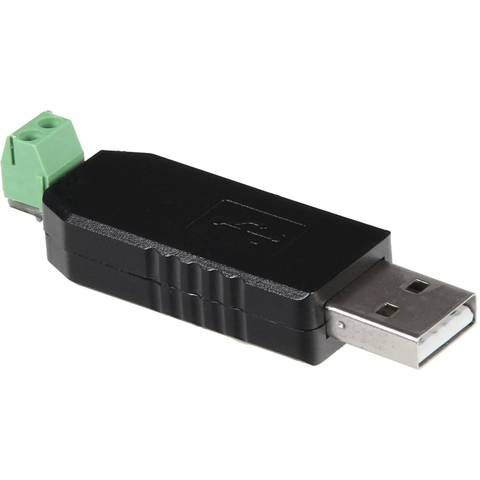
\includegraphics[width=0.4\textwidth]{assets/figures/Dimensionement/Convertisseur USB RS485.jpg}
    \caption{Convertisseur USB vers RS485 SBC-TTL-RS485 de Joy-IT \cite{joyit_sbc_ttl_rs485}}
    \label{fig:convertisseur_rs485}
\end{figure}
\begin{table}[H]
  \centering
  \caption{Caractéristiques du convertisseur USB-RS485 SBC-TTL-RS485}
  \label{tab:specs_rs485}
  \begin{tabular}{ll}
    \toprule
    \textbf{Paramètre} & \textbf{Valeur} \\
    \midrule
    Interface hôte & USB 2.0 type A \\
    Interface bus & RS485 (câble 2 fils) \\
    Alimentation & Bus USB (alimenté par l'hôte) \\
    Compatibilité & Raspberry Pi, Arduino, PC \\
    \bottomrule
  \end{tabular}
\end{table}
\subsection{Alimentation du moteur}
L'alimentation du moteur est assurée par le bloc secteur RS-25-24 (Mean Well) \cite{meanwell_rs2524}.
\subsubsection{Caractéristiques de l'alimentation}
\begin{figure}[H]
    \centering
    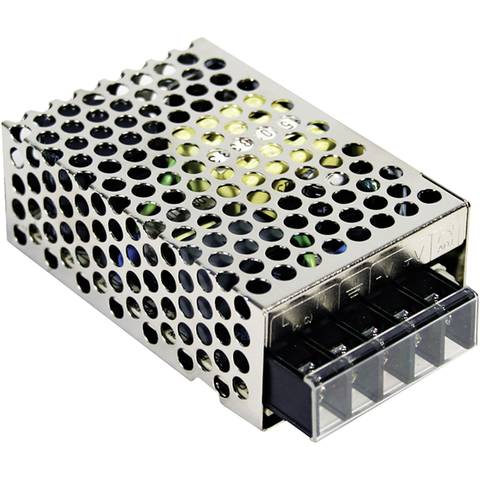
\includegraphics[width=0.4\textwidth]{assets/figures/Dimensionement/Alimentation moteur.jpg}
    \caption{Bloc d'alimentation à découpage RS-25-24 de Mean Well \cite{meanwell_rs2524}}
    \label{fig:alim_moteur}
\end{figure}
\begin{table}[H]
  \centering
  \caption{Caractéristiques de l'alimentation RS-25-24}
  \label{tab:specs_alim_moteur}
  \begin{tabular}{ll}
    \toprule
    \textbf{Paramètre} & \textbf{Valeur} \\
    \midrule
    Tension de sortie & $V_{\text{alim}} = 24$ V DC \\
    Courant maximal & $I_{\text{max}} = 1,1$ A \\
    Puissance maximale & 26 W \\
    \bottomrule
  \end{tabular}
\end{table}
\subsubsection{Vérification de la compatibilité}
La puissance disponible est :
\begin{equation}
    P_{\text{alim}} = V_{\text{alim}} \times I_{\text{max}} = 24 \times 1,1 = 26,4 \text{ W}
    \label{eq:puissance_alim}
\end{equation}
\noindent où $V_{\text{alim}} = 24$ V (tension de sortie) et $I_{\text{max}} = 1,1$ A (courant maximal disponible).
La puissance consommée par le moteur en fonctionnement nominal est :
\begin{equation}
    P_{\text{moteur}} = V_{\text{moteur}} \times I_{\text{moteur}} = 24 \times 0,42 = 10,1 \text{ W}
    \label{eq:puissance_moteur}
\end{equation}
\noindent où $V_{\text{moteur}} = 24$ V (tension moteur) et $I_{\text{moteur}} = 0,42$ A (courant nominal du moteur).
L'alimentation fournit donc une marge de sécurité de :
\begin{equation}
    \text{Marge} = \frac{P_{\text{alim}} - P_{\text{moteur}}}{P_{\text{alim}}} \times 100\% = \frac{26,4 - 10,1}{26,4} \times 100\% \approx 62\%
    \label{eq:marge_puissance}
\end{equation}
Cette marge permet d'accommoder des pics de consommation ou d'alimenter jusqu'à deux moteur simultanément.
\section{Système d'acquisition optique}
\subsection{Choix de la caméra}
\subsubsection{Dimensionnement et calcul de résolution}
La caméra doit assurer une détection fiable du fonctionnement du mouvement de montre. 
Pour ce faire, l'élément le plus fin à détecter est la largeur de l'aiguille des secondes, estimée à 0,15 mm. 
Pour garantir une détection fiable par traitement d'image, au moins 5 pixels doivent couvrir cette dimension.
La résolution requise est donc :
\begin{equation}
    R_{\text{requise}} = \frac{d_{\text{min}}}{N_{\text{pixels}}} = \frac{0,15}{5} = 0,030 \text{ mm/pixel}
    \label{eq:resolution_spatiale}
\end{equation}
\noindent où $d_{\text{min}}$ est la largeur minimale à détecter en $[mm]$ et $N_{\text{pixels}}$ est le nombre minimal de pixels requis sur cette distance.
Cela correspond à environ 33 pixels/mm. 
Le mouvement de montre le plus grand à observer fait $30$ mm de diamètre. 
On souhaite que la zone observée par la caméra soit légèrement plus large, soit $40 \times 40$ mm. 
Le nombre minimal de pixels du capteur en horizontal est donc :
\begin{equation}
    N_{\text{capteur}} = \frac{\text{Zone de travail}}{R_{\text{requise}}} = \frac{40}{0,030} \approx 1333 \text{ pixels}
    \label{eq:resolution_capteur}
\end{equation}
\noindent où Zone de travail = 40 mm (dimension du champ inspecté) et $R_{\text{requise}} = 0,030$ mm/pixel (résolution spatiale requise).
\subsubsection{Caméra sélectionnée}
Le modèle retenu est le VEN-505-36U3C-M01 \cite{va_imaging_ven505}, équipé d'un capteur Sony IMX335 de format 1/2,8". 
Cette résolution de 2592 x 1944 pixels (5 MP) dépasse largement l'exigence minimale de 1333 pixels, offrant une excellente marge de confort.
Ses caractéristiques principales sont présentées au tableau~\ref{tab:specs_camera}:
\begin{figure}[H]
    \centering
    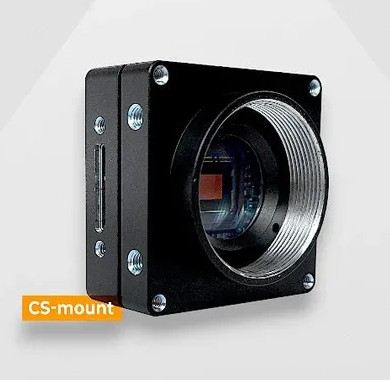
\includegraphics[width=0.4\textwidth]{assets/figures/Dimensionement/Camera.jpg}
    \caption{Caméra USB 3.0 5 MP VEN-505-36U3C-M01 \cite{va_imaging_ven505}}
    \label{fig:camera}
\end{figure}
\begin{table}[H]
  \centering
  \caption{Caractéristiques de la caméra VEN-505-36U3C-M01}
  \label{tab:specs_camera}
  \begin{tabular}{ll}
    \toprule
    \textbf{Paramètre} & \textbf{Valeur} \\
    \midrule
    Capteur & Sony IMX335 \\
    Format du capteur & 1/2,8" \\
    Résolution & 2592 x 1944 pixels (5 MP) \\
    Largeur du capteur & 5,37 mm \\
    Hauteur du capteur & 4,04 mm \\
    Interface & USB 3.0 \\
    Connecteur caméra & C-mount \\
    \bottomrule
  \end{tabular}
\end{table} 
\subsection{Choix de l'objectif}
\subsubsection{Dimensionnement de l'objectif}
La zone d'inspection souhaitée est un champ de $40 \times 40$ mm. 
Le grandissement optique nécessaire est déterminé par la dimension limitante (largeur du capteur par rapport à la largeur du champ) :
\begin{equation}
    m = \frac{W_{\text{capteur}}}{\text{Champ d'inspection}} = \frac{5,37}{40} = 0,134
    \label{eq:grandissement}
\end{equation}
\noindent où $W_{\text{capteur}} = 5,37$ mm (largeur du capteur) et Champ d'inspection = 40 mm.
La distance de travail est fixée à WD = 300 mm pour permettre un montage pratique du système de motorisation et d'éclairage. 
À partir du grandissement calculé et de cette distance de travail, la focale requise de l'objectif est déterminée par la relation de conjugaison pour un objectif à focale fixe :
\begin{equation}
    f = \frac{WD}{1 + \frac{1}{m}} = \frac{300}{1 + \frac{1}{0,134}} = \frac{300}{8,46} \approx 35,5 \text{ mm}
    \label{eq:focale}
\end{equation}
\noindent où WD = 300 mm (distance de travail) et $m = 0,134$ (grandissement).
Une focale de 35 mm est donc requise pour satisfaire ces contraintes.
\subsubsection{Objectif sélectionné}
L'objectif retenu est le VA-LCM-5MP-25MM-F2.0-018 \cite{va_imaging_lcm5mp}.
Ses caractéristiques principales sont présentées au tableau~\ref{tab:specs_objectif}:
\begin{figure}[H]
    \centering
    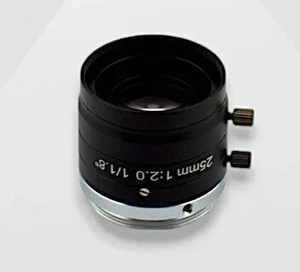
\includegraphics[width=0.4\textwidth]{assets/figures/Dimensionement/Objectif.jpg}
    \caption{Objectif C-mount VA-LCM-5MP-25MM-F2.0-018 \cite{va_imaging_lcm5mp}}
    \label{fig:objectif}
\end{figure}
\begin{table}[H]
  \centering
  \caption{Caractéristiques de l'objectif VA-LCM-5MP-25MM-F2.0-018}
  \label{tab:specs_objectif}
  \begin{tabular}{ll}
    \toprule
    \textbf{Paramètre} & \textbf{Valeur} \\
    \midrule
    Focale fixe & 25 mm \\
    Ouverture & F/2.0 \\
    Monture & C-mount \\
    Optimisation & Capteurs format 1" et 1/2,8" \\
    Distance de travail & 300 mm \\
    \bottomrule
  \end{tabular}
\end{table}
\subsubsection{Mise au point et profondeur de champ}
Les différents mouvements horlogers présentent des hauteurs totales variables (tableau~\ref{tab:dimensions_mouvements}), ce qui déplace axialement la face observée par la caméra d'un mouvement à l'autre.
Afin d'éviter de refaire la mise au point à chaque changement de mouvement, la profondeur de champ de l'objectif doit couvrir cet écart.
L'écart de hauteur totale entre le mouvement le plus épais (Mvt19, 8,73 mm) et le plus fin (Mvt111, 3,05 mm) vaut :
\begin{equation}
    \Delta h = h_{\text{max}} - h_{\text{min}} = 8,73 - 3,05 = 5,68 \text{ mm}
    \label{eq:delta_h_mouvements}
\end{equation}
La taille de pixel du capteur est déterminée à partir de sa largeur physique et de sa résolution horizontale :
\begin{equation}
    p = \frac{W_{\text{capteur}}}{N_{\text{pixels}}} = \frac{5,37}{2592} \approx 0,00207 \text{ mm} = 2,07~\mu\text{m}
    \label{eq:taille_pixel}
\end{equation}
En retenant un cercle de confusion égal à deux fois la taille d'un pixel, seuil couramment utilisé en vision industrielle pour définir la limite de flou acceptable, on obtient :
\begin{equation}
    c = 2p \approx 4,14~\mu\text{m} = 0,00414 \text{ mm}
    \label{eq:cercle_confusion}
\end{equation}
\noindent où $p = 2,07~\mu$m est la taille d'un pixel.
À partir de la focale $f = 25$ mm, de la distance de travail $do \approx 300$ mm et du nombre d'ouverture $N$ réglé par le diaphragme, la distance hyperfocale s'écrit :
\begin{equation}
    H(N) = f + \frac{f^2}{Nc}
    \label{eq:hyperfocale}
\end{equation}
\noindent d'où les limites de netteté proche et éloignée :
\begin{equation}
    D_n = \frac{H \cdot do}{H + (do - f)}
    \qquad
    D_f = \frac{H \cdot do}{H - (do - f)}
    \label{eq:limites_nettete}
\end{equation}
Avec l'ouverture native de l'objectif ($N = 2$, soit F/2.0), la profondeur de champ obtenue est :
\begin{equation}
    \text{DOF}(2) = D_f - D_n \approx 301,1 - 298,9 = 2,2 \text{ mm}
    \label{eq:dof_f2}
\end{equation}
\noindent ce qui est insuffisant pour couvrir l'écart $\Delta h = 5,68$ mm calculé précédemment : un réglage du diaphragme est donc nécessaire.
L'iris de l'objectif est gradué de F/2.0 à une position complètement fermée, l'avant-dernière graduation numérotée étant F/11.
La profondeur de champ maximale atteignable, obtenue à cette ouverture $N = 11$, vaut :
\begin{equation}
    \text{DOF}(11) = D_f - D_n \approx 306,1 - 294,1 = 12,0 \text{ mm}
    \label{eq:dof_f11}
\end{equation}
\noindent Cette profondeur de champ maximale de 12,0 mm dépasse largement l'écart $\Delta h = 5,68$ mm à couvrir : le système est donc compatible, avec une marge confortable, et il n'est pas nécessaire de refaire la mise au point d'un mouvement à l'autre.
En pratique, il n'est pas utile de fermer le diaphragme jusqu'à cette valeur extrême, ce qui limiterait inutilement la quantité de lumière atteignant le capteur.
En résolvant $\text{DOF}(N) = \Delta h$, on trouve $N \approx 5,2$, arrondi à la graduation normalisée $N = 5,6$ disponible sur l'objectif, pour laquelle :
\begin{equation}
    \text{DOF}(5,6) = D_f - D_n \approx 303,1 - 297,0 = 6,1 \text{ mm}
    \label{eq:dof_f56}
\end{equation}
\noindent ce qui couvre déjà la totalité de l'écart de hauteur entre mouvements.
Un réglage du diaphragme de F/2.0 à F/5.6 est donc retenu comme valeur de travail, suffisant pour conserver l'ensemble des mouvements du cahier des charges nets dans le champ de la caméra, quelle que soit leur hauteur totale.
La perte de luminosité associée à cette fermeture du diaphragme est compensée par la puissance disponible de la ring light (90 W), présentée à la section suivante.
\subsection{Système d'éclairage}
\subsubsection{Justification du choix d'une ring light}
L'observation du mouvement de montre en fonctionnement requiert un éclairage homogène et sans ombres. 
La ring light, montée coaxialement à l'objectif, fournit un éclairage diffus et uniforme du champ observé. 
À une distance de travail de 300 mm, un diamètre interne de 70 mm est requis pour ne pas obstruer le champ de vue de $40 \times 40$ mm. 
Un angle d'émission de 90° (horizontal) produit un éclairage rasant favorable à la mise en évidence des reliefs du mouvement.
\subsubsection{Ring light sélectionnée}
La ring light sélectionnée est le modèle VA-RL3-70-90W \cite{va_imaging_rl3}.
Ses caractéristiques principales sont présentées au tableau~\ref{tab:specs_ringlight}:
\begin{figure}[H]
    \centering
    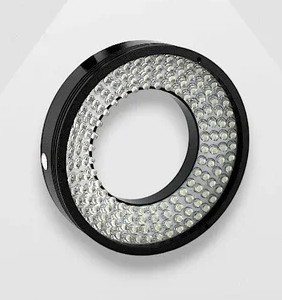
\includegraphics[width=0.4\textwidth]{assets/figures/Dimensionement/eclairage.jpg}
    \caption{Ring light industrielle VA-RL3-70-90W \cite{va_imaging_rl3}}
    \label{fig:ringlight}
\end{figure}
\begin{table}[H]
  \centering
  \caption{Caractéristiques de la ring light VA-RL3-70-90W}
  \label{tab:specs_ringlight}
  \begin{tabular}{ll}
    \toprule
    \textbf{Paramètre} & \textbf{Valeur} \\
    \midrule
    Diamètre interne & 70 mm \\
    Angle d'émission des LEDs & 90° (émission horizontale) \\
    Puissance & 90 W \\
    Type d'éclairage & Éclairage rasant \\
    Montage & Coaxial à l'objectif \\
    \bottomrule
  \end{tabular}
\end{table}
\subsubsection{Contrôleur d'éclairage}
Le contrôleur retenu est le VA-PS2-A4-60W-24V \cite{va_imaging_ps2}.
Ses caractéristiques principales sont présentées au tableau~\ref{tab:specs_controller}:
\begin{figure}[H]
    \centering
    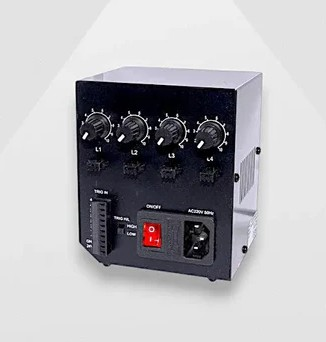
\includegraphics[width=0.4\textwidth]{assets/figures/Dimensionement/Alimentation eclairage.jpg}
    \caption{Contrôleur d'éclairage industriel VA-PS2-A4-60W-24V \cite{va_imaging_ps2}}
    \label{fig:controleur_eclairage}
\end{figure}
\begin{table}[H]
  \centering
  \caption{Caractéristiques du contrôleur VA-PS2-A4-60W-24V}
  \label{tab:specs_controller}
  \begin{tabular}{ll}
    \toprule
    \textbf{Paramètre} & \textbf{Valeur} \\
    \midrule
    Nombre de canaux & 4 canaux indépendants \\
    Tension d'alimentation & 24 V \\
    Puissance maximale & 60 W \\
    Réglage d'intensité & Gradateur intégré \\
    Entrée trigger & Oui \\
    Canaux utilisés dans ce projet & 1 canal \\
    \bottomrule
  \end{tabular}
\end{table}
\subsubsection{Filtration polarisante}
Les composants du mouvement de montre étant en métal poli, leur surface est fortement réfléchissante (réflexion spéculaire). 
Afin d'éliminer les reflets parasites et améliorer le contraste, une configuration en polarisation croisée est mise en place. 
Ce montage bloque la lumière directement réfléchie (composante spéculaire) et ne laisse passer que la composante diffuse, améliorant significativement le contraste de l'image. 
Cette configuration réduit le flux lumineux d'environ 20\%, ce qui est compensé par la puissance de la ring light (90 W).
Les composants optiques de filtration sélectionnés sont présentés au tableau~\ref{tab:specs_filters}:
\begin{figure}[H]
    \centering
    \begin{minipage}{0.45\textwidth}
        \centering
        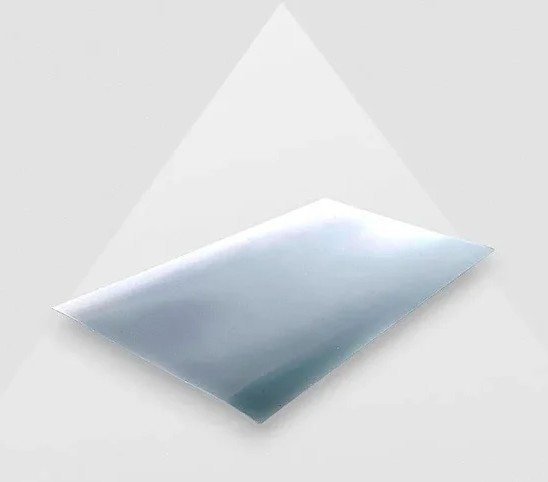
\includegraphics[width=\textwidth]{assets/figures/Dimensionement/feuille filtre polarisant.jpg}
    \end{minipage}
    \hfill
    \begin{minipage}{0.45\textwidth}
        \centering
        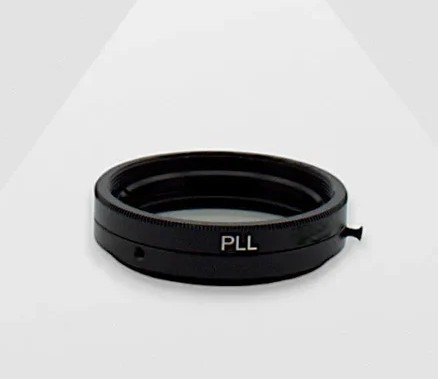
\includegraphics[width=\textwidth]{assets/figures/Dimensionement/filtre d'objectif polarisant.jpg}
    \end{minipage}
    \caption{Feuille polarisante VA-LFT-LPOL-300x200 (gauche) \cite{va_imaging_lft_sheet} et filtre polarisant d'objectif VA-LFT-LPOL-M35.5 (droite) \cite{va_imaging_lft_lens}}
    \label{fig:filtres_polarisants}
\end{figure}
\begin{table}[H]
  \centering
  \caption{Composants de filtration polarisante}
  \label{tab:specs_filters}
  \begin{tabular}{lll}
    \toprule
    \textbf{Composant} & \textbf{Référence} & \textbf{Fonction} \\
    \midrule
    Feuille polarisante & VA-LFT-LPOL-300x200 \cite{va_imaging_lft_sheet} & Devant ring light \\
    Filtre polarisant & VA-LFT-LPOL-M35.5 \cite{va_imaging_lft_lens} & Sur objectif (90°) \\
    \bottomrule
  \end{tabular}
\end{table}
\textbf{Résumé de l'acquisition~:} Le système optique offre une résolution de 15,4 $\mu$m/pixel sur un champ de 40 x 40 mm, avec une distance de travail de 300 mm et un éclairage rasant homogène. 
Ces caractéristiques permettent une détection fiable et reproductible du mouvement.



\section{Système d'accouplement fourche en T -- fourche en U}

L'accouplement entre la tige du mouvement horloger et l'arbre moteur est réalisé au moyen d'une fourche en T et d'une fourche en U (voir \autoref{fig:accouplement_proto}, section~\ref{sec:accouplement_fourche}).
La fourche en U, solidaire de l'arbre moteur, vient s'engager dans la fourche en T, dont les deux bras sont espacés de 25 mm, montée sur la tige du mouvement.
Ce principe d'accouplement à jeu angulaire transmet le couple de rotation tout en découplant les axes radiaux : les forces parasites susceptibles d'endommager le mouvement (charges radiales, bending) ne sont pas transmises, et une certaine tolérance au désalignement angulaire et radial est assurée naturellement par le jeu entre les deux fourches.

\subsection{Analyse de la saccade due au désalignement}

En revanche, un désalignement résiduel entre les deux axes introduit une variation périodique du rapport de transmission instantané, se traduisant par une légère saccade superposée au profil de vitesse théorique.
Pour un profil trapézoïdal 1/3–1/3–1/3 (accélération, vitesse constante, décélération), cette saccade se manifeste principalement en début et en fin de mouvement, là où la dérivée de vitesse est non nulle.
Afin de maintenir l'erreur de vitesse en dessous de 5 \%, le défaut d'alignement radial maximal admissible doit être rigoureusement contrôlé lors du montage.

\subsubsection{Analyse des tolérances de montage entre mouvements}

Les différents mouvements n'ayant pas les mêmes dimensions, la hauteur de la tige peut varier lors du montage dépendamment du mouvement.
\begin{align*}
  \text{Mouvement 1} &: 8{,}73 - 4{,}1 = 4{,}63\ \text{mm} \\
  \text{Mouvement 2} &: 7{,}23 - 2{,}8 = 4{,}43\ \text{mm} \\
  \text{Mouvement 3} &: 6{,}63 - 2{,}2 = 4{,}43\ \text{mm} \\
  \text{Mouvement 4} &: 8{,}63 - 4{,}2 = 4{,}43\ \text{mm} \\
  \text{Mouvement 5} &: 3{,}80 - 1{,}5 = 2{,}30\ \text{mm} \\
  \text{Mouvement 6} &: 3{,}05 - 1{,}0 = 2{,}05\ \text{mm} \\
  \text{Mouvement 7} &: 9{,}33 - 4{,}1 = 5{,}23\ \text{mm}
\end{align*}

La différence entre la hauteur maximale (Mouvement 7 : $5{,}23\ \text{mm}$) et minimale (Mouvement 6 : $2{,}05\ \text{mm}$) s'élève à :

\begin{equation}
  \Delta h = 5{,}23 - 2{,}05 = 3{,}18\ \text{mm}
  \label{eq:delta_h}
\end{equation}

Ce $\Delta h$ représente le désalignement radial réel maximal auquel
l'accouplement peut être soumis selon le mouvement monté. Il sert de valeur
de référence pour $e$ dans toute la suite de l'analyse.

\subsubsection{Modèle cinématique exact}

Le désalignement de l'accouplement est de nature \emph{radiale}~: les axes
moteur ($O_1$, fourche en U) et tige ($O_2$, fourche en T) restent
parallèles, mais décalés d'une distance $e$. Le point d'engagement entre les
deux fourches est entraîné à un rayon fixe $R = 12{,}5\ \text{mm}$ autour de
l'axe moteur $O_1$ (demi-écart de la fourche en T). La fourche en T, dont
l'axe $O_2$ est décalé de $e$ par rapport à $O_1$, « regarde » ce même point
d'engagement~: son orientation $\beta$ est donc l'angle, vu depuis $O_2$, du
point entraîné par le moteur à l'angle $\alpha$. Le point entraîné se trouve
en $(R\cos\alpha+e,\ R\sin\alpha)$ dans le repère centré sur $O_2$ ; son
angle $\beta$ vaut donc :

\begin{equation}
  \beta(\alpha) = \cos^{-1}\!\left(\frac{R\cos\alpha+e}{\sqrt{(R\cos\alpha+e)^2+(R\sin\alpha)^2}}\right)
  \label{eq:beta_alpha_cos}
\end{equation}

Cette forme en $\cos^{-1}$ ne renvoie toutefois que des valeurs dans
$[0°,180°]$ : au-delà de $\alpha=180°$, le signe correct de $\beta$ n'est
pas restitué. La forme équivalente suivante, utilisée pour les calculs et
les figures qui suivent, lève cette ambiguïté sur $[0°,360°[$ :

\begin{equation}
  \beta(\alpha) = \operatorname{atan2}\!\big(R\sin\alpha,\ e+R\cos\alpha\big)
  \qquad \alpha\in[0°,180°)
  \label{eq:beta_alpha}
\end{equation}

\paragraph{Symétrie de la fourche en T.} La fourche en T (tige) possède
\emph{deux} bras diamétralement opposés (espacés de 25~mm, donc $R$ de part
et d'autre de $O_2$) : ce n'est pas un point unique qui reste engagé sur un
tour complet, mais un bras qui entraîne la rotation sur un demi-tour moteur,
puis c'est le second bras -- géométriquement identique au premier, juste
tourné de 180° -- qui prend le relais et reproduit exactement le même
comportement. L'\eqref{eq:beta_alpha} n'est donc valable que sur un
demi-tour moteur ($\alpha\in[0°,180°)$) ; au-delà, elle se prolonge par
périodicité de 180°, et non de 360° :

\begin{equation}
  \beta(\alpha + 180°) = \beta(\alpha) + 180°
  \label{eq:beta_periodicity}
\end{equation}

La \autoref{fig:positions_angle} illustre cette géométrie tous les 45° sur un
tour complet, en reprenant la construction à deux cercles de rayon $R$ (un
autour de $O_1$, un autour de $O_2$) et en faisant apparaître le
désalignement $e$ entre les deux centres. Les deux points où le bras moteur
croiserait le cercle moteur sont toujours représentés (symétrie oblige)~;
celui qui est effectivement actif -- entouré sur la figure -- est en haut
pour $\alpha<180°$ et en bas pour $\alpha\geq180°$. On observe que les
panneaux de la seconde ligne ($225°$ à $315°$) reproduisent exactement les
mêmes valeurs de $\Delta$ que ceux de la première ligne ($45°$ à $135°$) :
c'est la périodicité de 180° de l'\eqref{eq:beta_periodicity}
(\autoref{fig:beta_evolution}, \autoref{fig:delta_evolution}).

\begin{figure}[H]
  \centering
  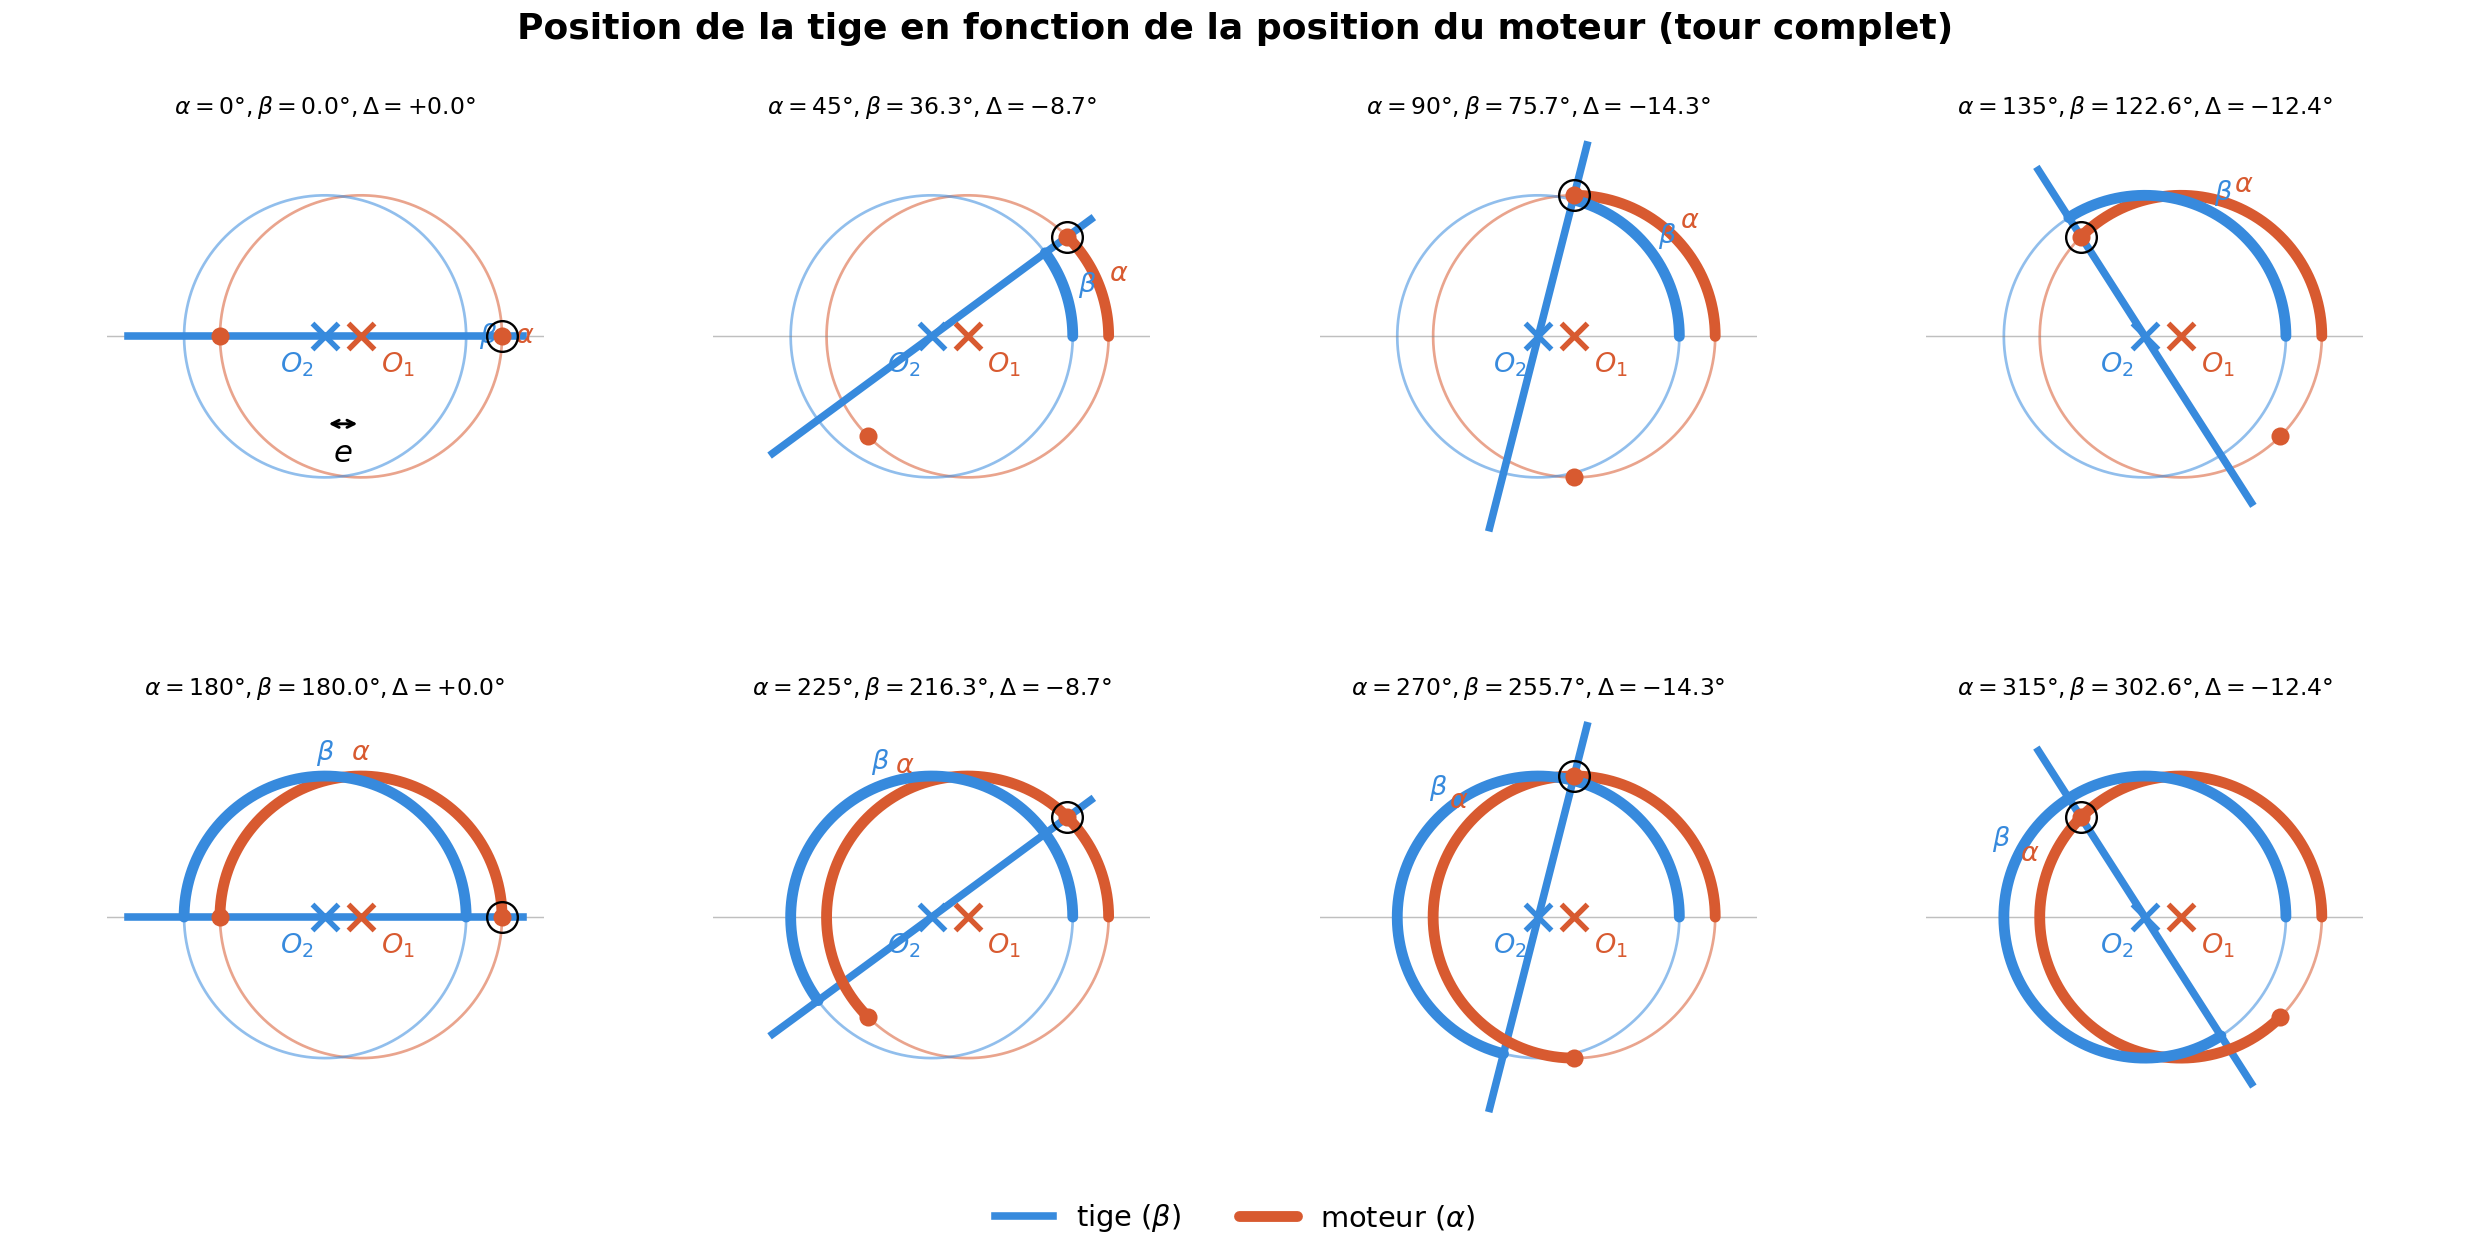
\includegraphics[width=\textwidth]{assets/figures/Implementation/fig_positions_angle.png}
  \caption{Position de la tige (bleu, angle $\beta$) en fonction de la
  position du moteur (orange, angle $\alpha$), tous les 45° sur un tour
  complet. Les axes $O_1$ (moteur) et $O_2$ (tige) et leur désalignement $e$
  sont indiqués sur le premier panneau ; le bras moteur actif est entouré.
  $R=12{,}5$~mm, $e=\Delta h=3{,}18$~mm.}
  \label{fig:positions_angle}
\end{figure}

\begin{figure}[H]
  \centering
  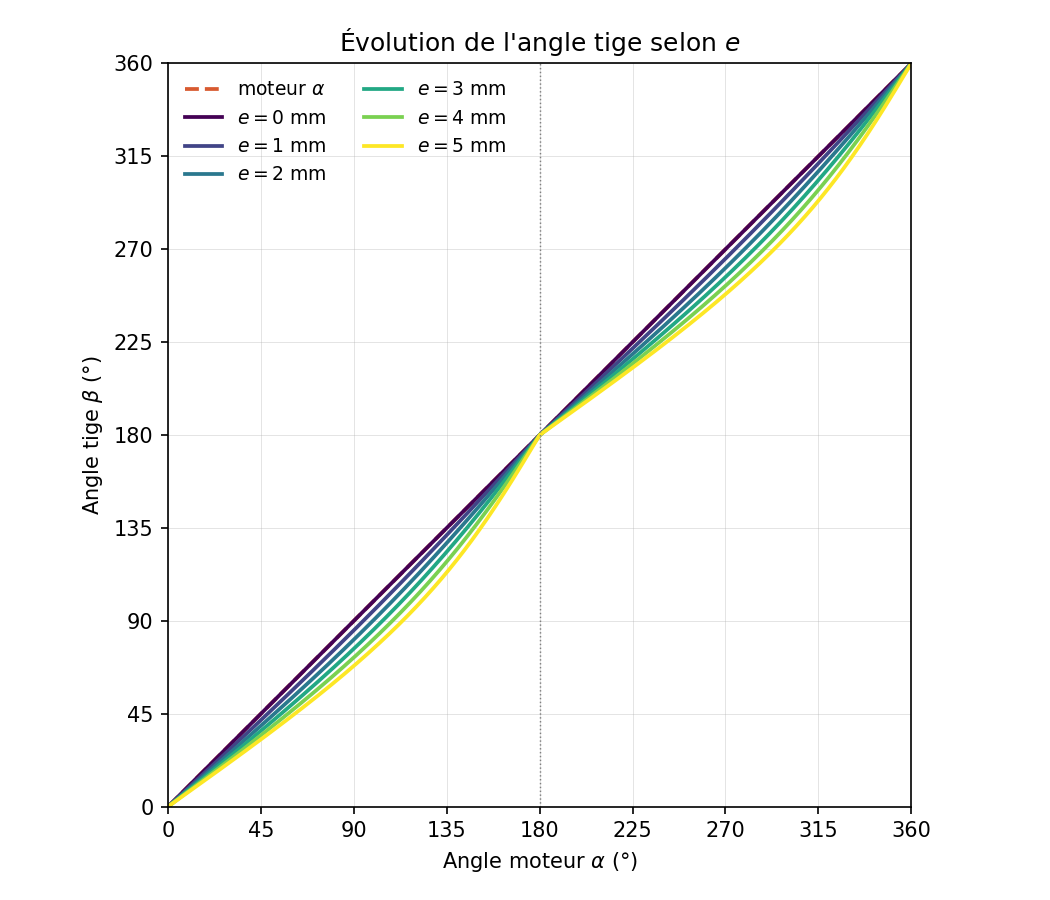
\includegraphics[width=0.75\textwidth]{assets/figures/Implementation/fig_beta_evolution.png}
  \caption{Évolution de l'angle tige $\beta$ sur un tour complet, pour
  différentes valeurs du désalignement $e$ (0 à 5~mm). Le désalignement réel
  ($\Delta h = 3{,}18$~mm) se situe entre les courbes $e=3$~mm et $e=4$~mm.
  La courbe présente un point anguleux à 180°, marquant le changement de
  bras actif.}
  \label{fig:beta_evolution}
\end{figure}

\begin{figure}[H]
  \centering
  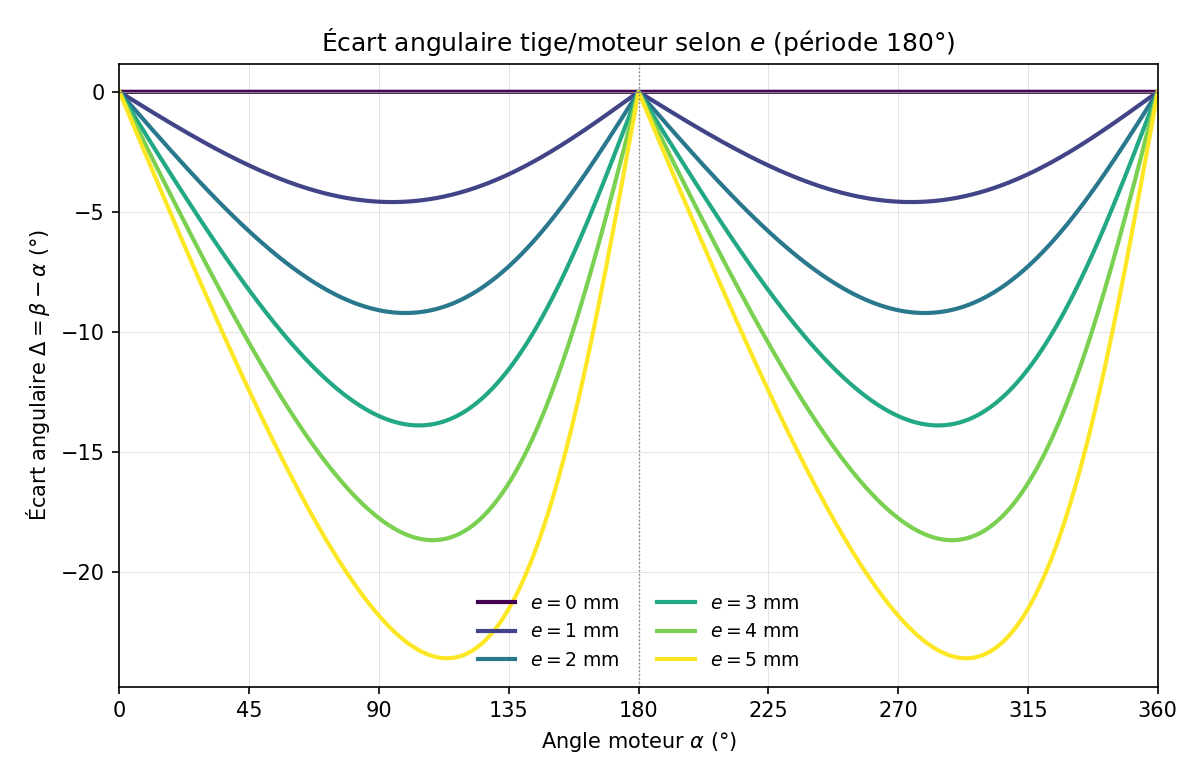
\includegraphics[width=0.8\textwidth]{assets/figures/Implementation/fig_delta_evolution.png}
  \caption{Écart angulaire $\Delta=\beta-\alpha$ sur un tour complet, pour
  différentes valeurs du désalignement $e$ (0 à 5~mm). Le motif se répète à
  l'identique tous les 180° (et non tous les 360°), conséquence directe de
  la symétrie de la fourche en T.}
  \label{fig:delta_evolution}
\end{figure}

\subsubsection{Erreur de vitesse}

En dérivant l'\eqref{eq:beta_alpha} par rapport à $\alpha$, on obtient le
rapport de transmission instantané exact, valable sur le même demi-tour
$\alpha\in[0°,180°)$ puis prolongé par périodicité de 180° comme
l'\eqref{eq:beta_periodicity} :

\begin{equation}
  \frac{\omega_2}{\omega_1} = \frac{d\beta}{d\alpha}
  = \frac{R(R+e\cos\alpha)}{R^2+e^2+2Re\cos\alpha}
  \label{eq:omega_ratio}
\end{equation}

L'erreur de vitesse relative $\varepsilon(\alpha) \equiv \omega_2/\omega_1-1$
s'écrit alors $\varepsilon(\alpha) = -e(e+R\cos\alpha)/(R^2+e^2+2Re\cos\alpha)$.
En posant $c=\cos\alpha$, on vérifie que $d\varepsilon/dc$ est du signe
constant de $-eR(R^2-e^2)$, indépendant de $c$~: $\varepsilon$ est donc
monotone en $\cos\alpha$, et ses extrema sont atteints aux bornes
$\alpha=0$ et $\alpha=\pi$ :

\begin{equation}
  \varepsilon_{\text{min}} = -\frac{e}{R+e} \quad (\alpha=0), \qquad
  \varepsilon_{\text{max}} = \frac{e}{R-e} \quad (\alpha=\pi)
  \label{eq:eps_bounds}
\end{equation}

Avec $e = \Delta h = 3{,}18\ \text{mm}$ et $R=12{,}5\ \text{mm}$ :

\begin{equation}
  \varepsilon_{\text{min}} = -\frac{3{,}18}{15{,}68} \approx -20{,}3\ \%, \qquad
  \varepsilon_{\text{max}} = \frac{3{,}18}{9{,}32} \approx 34{,}1\ \%
  \label{eq:eps_bounds_calc}
\end{equation}

Le maximum $\varepsilon_{\text{max}}$ est atteint à la borne $\alpha=180°$,
c'est-à-dire \emph{juste avant} le changement de bras actif~: $\beta$ reste
continue à cet instant (\autoref{fig:beta_evolution}), mais $d\beta/d\alpha$
y est discontinue, puisque le bras qui prend le relais redémarre son propre
cycle à $\varepsilon_{\text{min}}$. La vitesse de la tige subit donc un saut
brusque de $+34{,}1\ \%$ à $-20{,}3\ \%$ toutes les 180° de rotation moteur
(\autoref{fig:profil_saccade}), absorbé mécaniquement par le jeu angulaire de
l'accouplement mentionné plus haut.

\textbf{Ce résultat, obtenu à partir du modèle géométrique exact, est
nettement plus défavorable que le seuil de 5~\% envisagé initialement pour le
dimensionnement du jeu de l'accouplement.} Le rayon d'entraînement de
$12{,}5\ \text{mm}$ ne permet donc pas de garantir une erreur de vitesse
inférieure à 5~\% pour le désalignement réel observé entre mouvements
($\Delta h = 3{,}18$~mm) -- il faudrait pour cela un désalignement
$e \leq \varepsilon_{\text{seuil}}\cdot R/(1+\varepsilon_{\text{seuil}}) =
0{,}595\ \text{mm}$, très inférieur à $\Delta h$. Ce critère de 5~\% n'est
cependant qu'un indicateur intermédiaire~: ce qui importe réellement pour le
cahier des charges est l'imprécision de mesure qu'il engendre, analysée à la
\autoref{sec:precision_mesure}.

\subsubsection{Profil de vitesse simulé}

La \autoref{fig:profil_saccade} illustre, pour le désalignement réel
$e=\Delta h=3{,}18$~mm, la superposition de la saccade périodique
(\eqref{eq:omega_ratio}, prolongée par périodicité de 180° comme
l'\eqref{eq:beta_periodicity}) sur le profil de vitesse trapézoïdal
théorique de l'accouplement. Conformément à l'\eqref{eq:eps_bounds_calc}, la
vitesse instantanée croît jusqu'à $+34\ \%$ puis chute brusquement à
$-20\ \%$ à chaque changement de bras actif (tous les 180° de rotation
moteur, soit deux fois par tour), avant de recommencer le même cycle.

\begin{figure}[H]
  \centering
  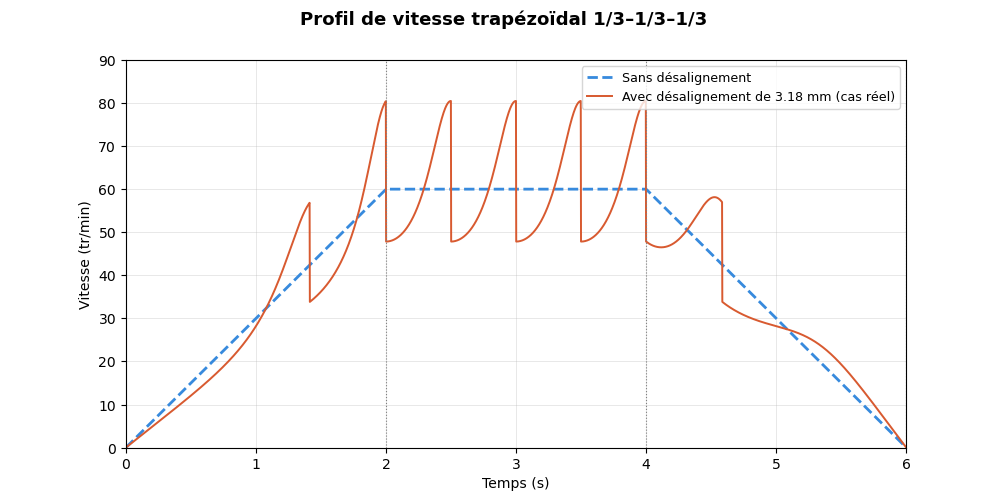
\includegraphics[width=0.85\textwidth]{assets/figures/Implementation/profil de vitesse trapezoidale avec saccade.png}
  \caption{Profil de vitesse trapézoïdal 1/3–1/3–1/3 avec saccade périodique due au désalignement réel de l'accouplement, $e=\Delta h=3{,}18$~mm. Le motif se répète tous les 180° de rotation moteur.}
  \label{fig:profil_saccade}
\end{figure}

\subsection{Analyse de la précision de la mesure}
\label{sec:precision_mesure}

Au-delà de la saccade de vitesse, le désalignement de l'accouplement
introduit également un déphasage angulaire entre le moteur et la tige du
mouvement. Ce déphasage est directement pertinent pour la précision de la
mesure de réserve de marche, puisque celle-ci est déduite du nombre de tours
effectués par la tige.

\subsubsection{Écart angulaire maximal entre moteur et mouvement}

L'écart angulaire $\Delta(\alpha) = \beta(\alpha)-\alpha$ est extrémal
lorsque $d\beta/d\alpha=1$, ce qui, d'après l'\eqref{eq:omega_ratio}, donne
la condition $\cos\alpha = -e/R$. En substituant cette valeur dans
l'\eqref{eq:beta_alpha}, le numérateur et le dénominateur de
$\operatorname{atan2}$ se simplifient en $R\sqrt{1-e^2/R^2}$ et $0$
respectivement, de sorte que $\beta=\pi/2$ \emph{exactement} en ce point~:
l'écart maximal se produit donc toujours lorsque la tige passe par 90°.
On en déduit l'écart angulaire maximal sous une forme remarquablement
simple :

\begin{equation}
  \Delta_{\text{max}} = \frac{\pi}{2} - \arccos\!\left(-\frac{e}{R}\right) = \arcsin\!\left(\frac{e}{R}\right)
  \label{eq:delta_max}
\end{equation}

Avec $e = \Delta h = 3{,}18\ \text{mm}$ et $R = 12{,}5\ \text{mm}$ :

\begin{equation}
  \Delta_{\text{max}} = \arcsin\!\left(\frac{3{,}18}{12{,}5}\right) \approx 14{,}74°
  \label{eq:delta_max_calc}
\end{equation}

Cette valeur, bien supérieure à l'estimation obtenue précédemment par
analogie avec un joint de Cardan, confirme qu'un modèle approché n'était pas
adapté ici~: le déphasage angulaire réel entre moteur et tige est de l'ordre
de $15°$, et non de $1°$.

Contrairement à $\varepsilon_{\text{max}}$ (\eqref{eq:eps_bounds_calc}),
atteint à la borne $\alpha=180°$ où le bras actif change,
$\Delta_{\text{max}}$ est atteint à l'intérieur du demi-tour
($\alpha\approx104{,}7°$, cf. $\cos\alpha=-e/R$) -- ce n'est donc pas un
artefact du changement de bras, mais un maximum lisse de l'écart de
position. Par périodicité (\eqref{eq:beta_periodicity}), cette même valeur
$\Delta_{\text{max}} = -14{,}74°$ est atteinte une seconde fois, à
$\alpha\approx284{,}7°$, avec le \emph{même signe} : la tige est toujours en
retard sur le moteur (jamais en avance) à ces deux instants, contrairement à
une oscillation symétrique $\pm\Delta_{\text{max}}$ que suggérerait une
périodicité de 360°. Seule l'amplitude \emph{maximale} de l'écart --
utilisée ci-dessous pour majorer l'imprécision de mesure -- est donc
inchangée par la prise en compte de la symétrie~; c'est sa fréquence
d'occurrence (deux fois par tour) et le signe constant qui diffèrent.

\subsubsection{Conversion en imprécision temporelle}

L'accouplement se situant sur la tige et non directement sur le
barillet, la conversion de $\Delta_{\text{max}}$ en temps doit passer par le
rapport de transmission $r$ (tige/barillet). Le nombre de tours de tige
nécessaires à un armage complet est :

\begin{equation}
  N_{\text{tige}} = r\cdot N_{\text{total}}
  \label{eq:n_tige}
\end{equation}

Ce nombre de tours de tige correspond, par définition, à la réserve de marche
totale $RM$ du mouvement (un armage complet fournit $RM$ heures de marche).
Un tour de tige (360°) équivaut donc à $RM/N_{\text{tige}}$ heures, soit
$3600\times RM/N_{\text{tige}}$ secondes, d'où l'équivalence angle--temps :

\begin{equation}
  1° \leftrightarrow \frac{RM}{N_{\text{tige}}}\times\frac{3600}{360}\ \text{s}
  = \frac{10\cdot RM}{N_{\text{tige}}}\ \text{s}
  \label{eq:conversion_deg_s}
\end{equation}

et l'imprécision de mesure induite par le désalignement s'écrit :

\begin{equation}
  \Delta t_{\text{max}} = \Delta_{\text{max}}[°] \times \frac{10\cdot RM}{N_{\text{tige}}}
  \label{eq:dt_max}
\end{equation}

Le cas le plus défavorable est le Mvt01 ($RM = 80$~h, $N_{\text{total}} =
10{,}3$~tr, $r = 3{,}33$). Par l'\eqref{eq:n_tige} :

\begin{equation}
  N_{\text{tige}} = 3{,}33\times 10{,}3 \approx 34{,}30\ \text{tr}
  \label{eq:n_tige_mvt01}
\end{equation}

puis, par l'\eqref{eq:dt_max} avec $\Delta_{\text{max}} = 14{,}74°$
(\eqref{eq:delta_max_calc}) :

\begin{equation}
  \Delta t_{\text{max}} = 14{,}74\times\frac{10\times 80}{34{,}30} = 14{,}74\times 23{,}32 \approx 344\ \text{s} \approx 5{,}73\ \text{min}
  \label{eq:dt_max_mvt01}
\end{equation}

\subsubsection{Désalignement limite pour respecter l'exigence E2}

L'exigence \textbf{E2} du cahier des charges impose une précision de mesure
$\leq 15\ \text{min}$. En inversant l'\eqref{eq:dt_max} (avec
l'\eqref{eq:delta_max}), on obtient le désalignement radial $e$ qui amènerait
$\Delta t_{\text{max}}$ exactement à cette limite, pour le cas le plus
défavorable (Mvt01) :

\begin{equation}
  e_{15\text{min}} = R\sin\!\left(\frac{15\times 60}{10\cdot RM/N_{\text{tige}}}\right)
  = 12{,}5\times\sin(38{,}59°) \approx 7{,}80\ \text{mm}
  \label{eq:e_15min}
\end{equation}

La \autoref{fig:precision_e_limite} illustre, pour le mouvement Mvt01,
l'imprécision de mesure obtenue sur un tour complet du moteur, pour le
désalignement réel ($e=3{,}18$~mm) et pour ce désalignement limite
($e=7{,}80$~mm). Conformément à la périodicité de 180°, chaque courbe
redescend deux fois par tour~: la courbe orange touche tout juste $-15$~min
à ces deux occasions, tandis que la courbe bleue (cas réel) ne descend qu'à
environ $-5{,}7$~min, soit une marge de \SI{4.62}{\mm} (59~\%) sur le
désalignement admissible.

\begin{figure}[H]
  \centering
  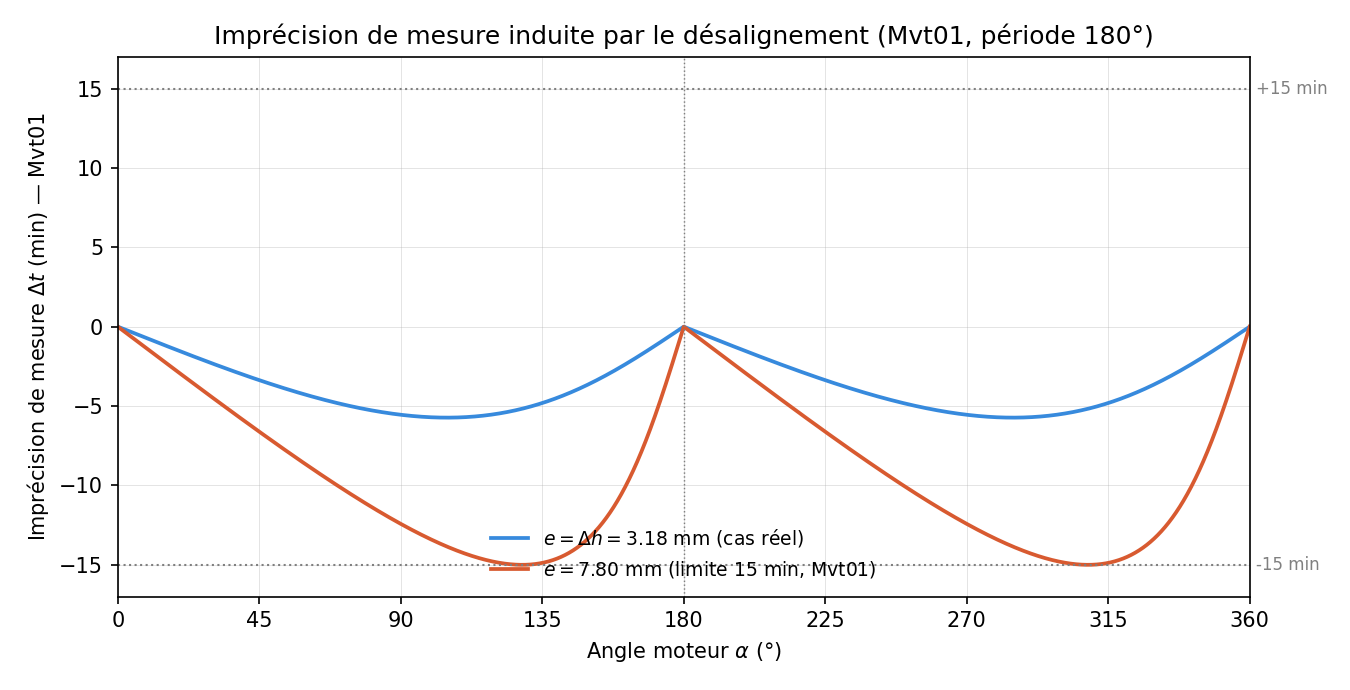
\includegraphics[width=0.9\textwidth]{assets/figures/Implementation/fig_precision_e_limite.png}
  \caption{Imprécision de mesure sur un tour moteur complet pour le Mvt01
  (cas le plus défavorable), au désalignement réel ($e=3{,}18$~mm) et au
  désalignement limite pour l'exigence E2 ($e=7{,}80$~mm). Le motif se
  répète tous les 180° de rotation moteur.}
  \label{fig:precision_e_limite}
\end{figure}

\subsubsection{Application à tous les mouvements}

Le \autoref{tab:precision_desalignement} reprend, selon la même démarche
(\eqref{eq:n_tige}, \eqref{eq:dt_max} et \eqref{eq:e_15min}), les résultats
pour l'ensemble des mouvements, avec $\Delta_{\text{max}} = 14{,}74°$
(\eqref{eq:delta_max_calc}, indépendant du mouvement puisqu'il ne dépend que
de $e$ et $R$).

\begin{table}[H]
  \centering
  \caption{Imprécision de mesure induite par le désalignement réel ($e=\Delta h=3{,}18$~mm) et désalignement limite pour l'exigence E2 (15 min)}
  \label{tab:precision_desalignement}
  \begin{tabular}{|c|c|c|c|c|c|}
    \hline
    \textbf{Mouvement} & $\boldsymbol{RM}$ \textbf{[h]} & $\boldsymbol{N_{\text{tige}}}$ \textbf{[tr]} & $\boldsymbol{\Delta t_{\text{max}}}$ \textbf{[min]} & \textbf{Marge} & $\boldsymbol{e_{15\text{min}}}$ \textbf{[mm]} \\
    \hline
    Mvt19             & 100 & 47{,}12 & 5{,}21 & 65\,\% & 8{,}43 \\
    Mvt01             & 80  & 34{,}30 & 5{,}73 & 62\,\% & 7{,}80 \\
    Mvt200 / Mvt200.1 & 90  & 43{,}96 & 5{,}03 & 66\,\% & 8{,}68 \\
    Mvt110            & 90  & 68{,}16 & 3{,}24 & 78\,\% & 11{,}60 \\
    Mvt111            & 89  & 41{,}44 & 5{,}28 & 65\,\% & 8{,}35 \\
    \hline
  \end{tabular}
\end{table}

L'imprécision de mesure induite par le désalignement réel de l'accouplement
reste comprise entre $3{,}2$ et $5{,}7$ minutes selon le mouvement, ce qui
respecte l'exigence de précision \textbf{E2 (\SI{15}{\minute})} du cahier des
charges, mais avec une marge nettement plus restreinte (62 à 78~\%) que ce
qu'une analyse au premier ordre aurait suggéré. Le mouvement Mvt01 est le
cas le plus contraignant, avec seulement \SI{4.62}{\mm} de marge sur le
désalignement admissible avant de dépasser l'exigence E2. Le désalignement
mécanique de l'accouplement reste donc acceptable pour le système, mais ne
doit pas être négligé lors du montage~: un contrôle plus rigoureux de $\Delta h$
serait souhaitable pour préserver cette marge.

\subsection{Analyse des contraintes et déformations}

\subsubsection{Données du problème}

La masse rapportée en bout de tige est un cylindre de fonte grise ($\rho = 7{,}2\ \text{g/cm}^3$) d'un volume de $825{,}35\ \text{mm}^3$, ce qui donne une masse de :

\[
  m = \rho \cdot V = 7{,}2 \times 10^{-3} \times 825{,}35 \times 10^{-3} = 5{,}94\ \text{g}
\]

La tige est modélisée comme une poutre encastrée-libre en acier inoxydable ($E = 200\ \text{GPa}$), de diamètre $d = 1{,}2\ \text{mm}$ et de longueur $L = 10{,}75\ \text{mm}$.

\subsubsection{Propriétés de la section transversale}

Le moment quadratique et le module de résistance d'une section circulaire pleine sont :

\[
  I = \frac{\pi d^4}{64} = \frac{\pi \times 1{,}2^4}{64} \approx 0{,}1018\ \text{mm}^4
  \qquad
  W = \frac{\pi d^3}{32} \approx 0{,}1696\ \text{mm}^3
\]

\subsubsection{Efforts générés}

La force appliquée en bout correspond au poids de la masse :

\[
  F = m \cdot g = 5{,}94 \times 10^{-3} \times 9{,}81 \approx 58{,}3\ \text{mN}
\]

Le moment fléchissant maximal, situé à l'encastrement, vaut :

\[
  M_{max} = F \cdot L = 58{,}3 \times 10^{-3} \times 10{,}75 \approx 0{,}627\ \text{N{\cdot}mm}
\]

\subsubsection{Flèche en bout de tige}

En appliquant la formule de la poutre encastrée chargée en bout :

\[
  f = \frac{F L^3}{3EI}
  = \frac{58{,}3 \times 10^{-3} \times 10{,}75^3}{3 \times 200\,000 \times 0{,}1018}
  \approx 3{,}8 \times 10^{-3}\ \mu\text{m}
\]

La déflexion est donc de l'ordre du nanomètre, ce qui est négligeable au regard de toute tolérance mécanique en horlogerie.

\subsubsection{Contrainte de flexion}

La contrainte normale maximale, à l'encastrement, est :

\[
  \sigma_{max} = \frac{M_{max}}{W} = \frac{0{,}627}{0{,}1696} \approx 3{,}7 \times 10^{-3}\ \text{MPa}
\]

La limite élastique d'un acier inoxydable courant étant de l'ordre de $300\ \text{MPa}$, la marge de sécurité est supérieure à $\times 80\,000$. La tige ne présente aucun risque de déformation plastique.
